% =====================================================================
%  Can a Quantum Kernel Pick Better Demonstrations?
%  Venue-neutral source. The template (IEEE, Springer LNCS, ACM or a plain arXiv layout) is chosen by
%  ONE line in configs/config.yaml (paper: venue:) and written into venue.tex and authors.tex by
%      python -m src.pipeline paper
%  Every number (\R...) and every result sentence (\T...) is written by the same command into
%  results_macros.tex and results_text.tex. Compile with  latexmk -pdf main.tex  or on Overleaf.
% =====================================================================
% Written by src/paper_text.py: template 'ieee' (configs/config.yaml, paper: venue:).
\documentclass[conference]{IEEEtran}
\IEEEoverridecommandlockouts
\usepackage{cite}
\usepackage[hidelinks]{hyperref}
\newtheorem{proposition}{Proposition}
\newenvironment{paperproof}{\begin{IEEEproof}}{\end{IEEEproof}}
\newcommand{\PaperBibStyle}{IEEEtran}
\newcommand{\makefront}{\maketitle\begin{abstract}\PaperAbstract\end{abstract}%
\begin{IEEEkeywords}\PaperKeywords\end{IEEEkeywords}}
\newcommand{\makefrontplain}{\maketitle}
\newcommand{\paperack}[1]{\section*{Acknowledgment}#1}

\usepackage{amsmath,amssymb,amsfonts}
\usepackage{graphicx}
\usepackage{booktabs}
\usepackage{multirow}
\usepackage{xcolor}
\usepackage{tikz}
\usetikzlibrary{positioning,arrows.meta,fit,backgrounds,calc}
\usepackage{quantikz}
\usepackage{url}

% ---- result numbers and sentences --------------------------------------
\newcommand{\res}[1]{#1}
% Written by src/paper_tables.py. Do not edit by hand: rerun  python -m src.pipeline paper
\providecommand{\res}[1]{#1}
\newcommand{\RAblAngle}{\res{\textbf{XYZ}}}
\newcommand{\RAblCos}{\res{\textbf{XYZ}}}
\newcommand{\RAblNoStd}{\res{\textbf{XYZ}}}
\newcommand{\RAblNoTune}{\res{\textbf{XYZ}}}
\newcommand{\RAblPca}{\res{\textbf{XYZ}}}
\newcommand{\RAblProj}{\res{\textbf{XYZ}}}
\newcommand{\RAblRbf}{\res{\textbf{XYZ}}}
\newcommand{\RAblRbfPca}{\res{\textbf{XYZ}}}
\newcommand{\RAblRepOne}{\res{\textbf{XYZ}}}
\newcommand{\RAblRepThree}{\res{\textbf{XYZ}}}
\newcommand{\RAblShots}{\res{\textbf{XYZ}}}
\newcommand{\RAblTrunc}{\res{\textbf{XYZ}}}
\newcommand{\RBankCIIqpRbfMain}{\res{\textbf{XYZ}}}
\newcommand{\RBankCIIqpRbfOpen}{\res{\textbf{XYZ}}}
\newcommand{\RBankCITrainedMain}{\res{\textbf{XYZ}}}
\newcommand{\RBankCITrainedOpen}{\res{\textbf{XYZ}}}
\newcommand{\RBankEquivIqpRbfMain}{\res{\textbf{XYZ}}}
\newcommand{\RBankEquivIqpRbfOpen}{\res{\textbf{XYZ}}}
\newcommand{\RBankEquivTrainedMain}{\res{\textbf{XYZ}}}
\newcommand{\RBankEquivTrainedOpen}{\res{\textbf{XYZ}}}
\newcommand{\RBankGapIqpRbfMain}{\res{\textbf{XYZ}}}
\newcommand{\RBankGapIqpRbfOpen}{\res{\textbf{XYZ}}}
\newcommand{\RBankGapTrainedMain}{\res{\textbf{XYZ}}}
\newcommand{\RBankGapTrainedOpen}{\res{\textbf{XYZ}}}
\newcommand{\RBankHeadroomMain}{\res{\textbf{XYZ}}}
\newcommand{\RBankHeadroomOpen}{\res{\textbf{XYZ}}}
\newcommand{\RBankMainAccRandom}{\res{\textbf{XYZ}}}
\newcommand{\RBankMainAccBm}{\res{\textbf{XYZ}}}
\newcommand{\RBankMainAccMmrCos}{\res{\textbf{XYZ}}}
\newcommand{\RBankMainAccNca}{\res{\textbf{XYZ}}}
\newcommand{\RBankMainAccOracle}{\res{\textbf{XYZ}}}
\newcommand{\RBankMainAccQTrained}{\res{\textbf{XYZ}}}
\newcommand{\RBankMainAccRbfTrained}{\res{\textbf{XYZ}}}
\newcommand{\RBankMainAccCosFull}{\res{\textbf{XYZ}}}
\newcommand{\RBankMainAccCosLda}{\res{\textbf{XYZ}}}
\newcommand{\RBankMainAccRbf}{\res{\textbf{XYZ}}}
\newcommand{\RBankMainAccAngle}{\res{\textbf{XYZ}}}
\newcommand{\RBankMainAccIqp}{\res{\textbf{XYZ}}}
\newcommand{\RBankMainAccProj}{\res{\textbf{XYZ}}}
\newcommand{\RBankOpenAccRandom}{\res{\textbf{XYZ}}}
\newcommand{\RBankOpenAccBm}{\res{\textbf{XYZ}}}
\newcommand{\RBankOpenAccMmrCos}{\res{\textbf{XYZ}}}
\newcommand{\RBankOpenAccNca}{\res{\textbf{XYZ}}}
\newcommand{\RBankOpenAccOracle}{\res{\textbf{XYZ}}}
\newcommand{\RBankOpenAccQTrained}{\res{\textbf{XYZ}}}
\newcommand{\RBankOpenAccRbfTrained}{\res{\textbf{XYZ}}}
\newcommand{\RBankOpenAccCosFull}{\res{\textbf{XYZ}}}
\newcommand{\RBankOpenAccCosLda}{\res{\textbf{XYZ}}}
\newcommand{\RBankOpenAccRbf}{\res{\textbf{XYZ}}}
\newcommand{\RBankOpenAccAngle}{\res{\textbf{XYZ}}}
\newcommand{\RBankOpenAccIqp}{\res{\textbf{XYZ}}}
\newcommand{\RBankOpenAccProj}{\res{\textbf{XYZ}}}
\newcommand{\RBestRealDbpediaMain}{\res{\textbf{XYZ}}}
\newcommand{\RBestRealDbpediaOpen}{\res{\textbf{XYZ}}}
\newcommand{\RBestRealEmotionMain}{\res{\textbf{XYZ}}}
\newcommand{\RBestRealEmotionOpen}{\res{\textbf{XYZ}}}
\newcommand{\RBestRealTrecMain}{\res{\textbf{XYZ}}}
\newcommand{\RBestRealTrecOpen}{\res{\textbf{XYZ}}}
\newcommand{\RBwAllWithin}{\res{\textbf{XYZ}}}
\newcommand{\RBwChanged}{\res{\textbf{XYZ}}}
\newcommand{\RBwGapAtLlmC}{\res{\textbf{XYZ}}}
\newcommand{\RBwMaxGap}{\res{\textbf{XYZ}}}
\newcommand{\RBwSettings}{\res{\textbf{XYZ}}}
\newcommand{\RCIDbpediaMain}{\res{\textbf{XYZ}}}
\newcommand{\RCIDbpediaOpen}{\res{\textbf{XYZ}}}
\newcommand{\RCIEmotionMain}{\res{\textbf{XYZ}}}
\newcommand{\RCIEmotionOpen}{\res{\textbf{XYZ}}}
\newcommand{\RCITrecMain}{\res{\textbf{XYZ}}}
\newcommand{\RCITrecOpen}{\res{\textbf{XYZ}}}
\newcommand{\RDbpediaAccRandom}{\res{\textbf{XYZ}}}
\newcommand{\RDbpediaAccBm}{\res{\textbf{XYZ}}}
\newcommand{\RDbpediaAccMmrCos}{\res{\textbf{XYZ}}}
\newcommand{\RDbpediaAccMmrIqp}{\res{\textbf{XYZ}}}
\newcommand{\RDbpediaAccNca}{\res{\textbf{XYZ}}}
\newcommand{\RDbpediaAccOracle}{\res{\textbf{XYZ}}}
\newcommand{\RDbpediaAccFusion}{\res{\textbf{XYZ}}}
\newcommand{\RDbpediaAccQTrained}{\res{\textbf{XYZ}}}
\newcommand{\RDbpediaAccRbfTrained}{\res{\textbf{XYZ}}}
\newcommand{\RDbpediaAccCosFull}{\res{\textbf{XYZ}}}
\newcommand{\RDbpediaAccCosLda}{\res{\textbf{XYZ}}}
\newcommand{\RDbpediaAccEuclid}{\res{\textbf{XYZ}}}
\newcommand{\RDbpediaAccRbf}{\res{\textbf{XYZ}}}
\newcommand{\RDbpediaAccAngle}{\res{\textbf{XYZ}}}
\newcommand{\RDbpediaAccIqp}{\res{\textbf{XYZ}}}
\newcommand{\RDbpediaAccProj}{\res{\textbf{XYZ}}}
\newcommand{\RDiffCIEasyDbpedia}{\res{\textbf{XYZ}}}
\newcommand{\RDiffCIEasyEmotion}{\res{\textbf{XYZ}}}
\newcommand{\RDiffCIEasyTrec}{\res{\textbf{XYZ}}}
\newcommand{\RDiffCIHardDbpedia}{\res{\textbf{XYZ}}}
\newcommand{\RDiffCIHardEmotion}{\res{\textbf{XYZ}}}
\newcommand{\RDiffCIHardTrec}{\res{\textbf{XYZ}}}
\newcommand{\RDiffEasyDbpedia}{\res{\textbf{XYZ}}}
\newcommand{\RDiffEasyEmotion}{\res{\textbf{XYZ}}}
\newcommand{\RDiffEasyTrec}{\res{\textbf{XYZ}}}
\newcommand{\RDiffHardDbpedia}{\res{\textbf{XYZ}}}
\newcommand{\RDiffHardEmotion}{\res{\textbf{XYZ}}}
\newcommand{\RDiffHardTrec}{\res{\textbf{XYZ}}}
\newcommand{\REmotionAccRandom}{\res{\textbf{XYZ}}}
\newcommand{\REmotionAccBm}{\res{\textbf{XYZ}}}
\newcommand{\REmotionAccMmrCos}{\res{\textbf{XYZ}}}
\newcommand{\REmotionAccMmrIqp}{\res{\textbf{XYZ}}}
\newcommand{\REmotionAccNca}{\res{\textbf{XYZ}}}
\newcommand{\REmotionAccOracle}{\res{\textbf{XYZ}}}
\newcommand{\REmotionAccFusion}{\res{\textbf{XYZ}}}
\newcommand{\REmotionAccQTrained}{\res{\textbf{XYZ}}}
\newcommand{\REmotionAccRbfTrained}{\res{\textbf{XYZ}}}
\newcommand{\REmotionAccCosFull}{\res{\textbf{XYZ}}}
\newcommand{\REmotionAccCosLda}{\res{\textbf{XYZ}}}
\newcommand{\REmotionAccEuclid}{\res{\textbf{XYZ}}}
\newcommand{\REmotionAccRbf}{\res{\textbf{XYZ}}}
\newcommand{\REmotionAccAngle}{\res{\textbf{XYZ}}}
\newcommand{\REmotionAccIqp}{\res{\textbf{XYZ}}}
\newcommand{\REmotionAccProj}{\res{\textbf{XYZ}}}
\newcommand{\REquivMargin}{\res{2}}
\newcommand{\REquivMmrIqpvsMmrCosDbpedia}{\res{\textbf{XYZ}}}
\newcommand{\REquivMmrIqpvsMmrCosEmotion}{\res{\textbf{XYZ}}}
\newcommand{\REquivMmrIqpvsMmrCosTrec}{\res{\textbf{XYZ}}}
\newcommand{\REquivFusionvsCosFullDbpedia}{\res{\textbf{XYZ}}}
\newcommand{\REquivFusionvsCosFullEmotion}{\res{\textbf{XYZ}}}
\newcommand{\REquivFusionvsCosFullTrec}{\res{\textbf{XYZ}}}
\newcommand{\REquivQTrainedvsRbfTrainedDbpedia}{\res{\textbf{XYZ}}}
\newcommand{\REquivQTrainedvsRbfTrainedEmotion}{\res{\textbf{XYZ}}}
\newcommand{\REquivQTrainedvsRbfTrainedTrec}{\res{\textbf{XYZ}}}
\newcommand{\REquivQTrainedvsIqpDbpedia}{\res{\textbf{XYZ}}}
\newcommand{\REquivQTrainedvsIqpEmotion}{\res{\textbf{XYZ}}}
\newcommand{\REquivQTrainedvsIqpTrec}{\res{\textbf{XYZ}}}
\newcommand{\REquivIqpvsNcaDbpedia}{\res{\textbf{XYZ}}}
\newcommand{\REquivIqpvsNcaEmotion}{\res{\textbf{XYZ}}}
\newcommand{\REquivIqpvsNcaTrec}{\res{\textbf{XYZ}}}
\newcommand{\REquivIqpvsCosFullDbpedia}{\res{\textbf{XYZ}}}
\newcommand{\REquivIqpvsCosFullEmotion}{\res{\textbf{XYZ}}}
\newcommand{\REquivIqpvsCosFullTrec}{\res{\textbf{XYZ}}}
\newcommand{\REquivIqpvsCosLdaDbpedia}{\res{\textbf{XYZ}}}
\newcommand{\REquivIqpvsCosLdaEmotion}{\res{\textbf{XYZ}}}
\newcommand{\REquivIqpvsCosLdaTrec}{\res{\textbf{XYZ}}}
\newcommand{\REquivIqpvsRbfDbpedia}{\res{\textbf{XYZ}}}
\newcommand{\REquivIqpvsRbfEmotion}{\res{\textbf{XYZ}}}
\newcommand{\REquivIqpvsRbfTrec}{\res{\textbf{XYZ}}}
\newcommand{\REquivProjvsRbfDbpedia}{\res{\textbf{XYZ}}}
\newcommand{\REquivProjvsRbfEmotion}{\res{\textbf{XYZ}}}
\newcommand{\REquivProjvsRbfTrec}{\res{\textbf{XYZ}}}
\newcommand{\RGapDbpediaMain}{\res{\textbf{XYZ}}}
\newcommand{\RGapDbpediaOpen}{\res{\textbf{XYZ}}}
\newcommand{\RGapEmotionMain}{\res{\textbf{XYZ}}}
\newcommand{\RGapEmotionOpen}{\res{\textbf{XYZ}}}
\newcommand{\RGapTrecMain}{\res{\textbf{XYZ}}}
\newcommand{\RGapTrecOpen}{\res{\textbf{XYZ}}}
\newcommand{\RHeadroomDbpediaMain}{\res{\textbf{XYZ}}}
\newcommand{\RHeadroomDbpediaOpen}{\res{\textbf{XYZ}}}
\newcommand{\RHeadroomEmotionMain}{\res{\textbf{XYZ}}}
\newcommand{\RHeadroomEmotionOpen}{\res{\textbf{XYZ}}}
\newcommand{\RHeadroomIqpDbpediaMain}{\res{\textbf{XYZ}}}
\newcommand{\RHeadroomIqpDbpediaOpen}{\res{\textbf{XYZ}}}
\newcommand{\RHeadroomIqpEmotionMain}{\res{\textbf{XYZ}}}
\newcommand{\RHeadroomIqpEmotionOpen}{\res{\textbf{XYZ}}}
\newcommand{\RHeadroomIqpTrecMain}{\res{\textbf{XYZ}}}
\newcommand{\RHeadroomIqpTrecOpen}{\res{\textbf{XYZ}}}
\newcommand{\RHeadroomTrecMain}{\res{\textbf{XYZ}}}
\newcommand{\RHeadroomTrecOpen}{\res{\textbf{XYZ}}}
\newcommand{\RHwBackend}{\res{\textbf{XYZ}}}
\newcommand{\RHwErr}{\res{\textbf{XYZ}}}
\newcommand{\RHwJ}{\res{\textbf{XYZ}}}
\newcommand{\RHwRank}{\res{\textbf{XYZ}}}
\newcommand{\RJRbfAngleDbpedia}{\res{\textbf{XYZ}}}
\newcommand{\RJRbfAngleEmotion}{\res{\textbf{XYZ}}}
\newcommand{\RJRbfAngleMax}{\res{\textbf{XYZ}}}
\newcommand{\RJRbfAngleMin}{\res{\textbf{XYZ}}}
\newcommand{\RJRbfAngleTrec}{\res{\textbf{XYZ}}}
\newcommand{\RJRbfIqpDbpedia}{\res{\textbf{XYZ}}}
\newcommand{\RJRbfIqpEmotion}{\res{\textbf{XYZ}}}
\newcommand{\RJRbfIqpMax}{\res{\textbf{XYZ}}}
\newcommand{\RJRbfIqpMin}{\res{\textbf{XYZ}}}
\newcommand{\RJRbfIqpTrec}{\res{\textbf{XYZ}}}
\newcommand{\RJShotsDbpedia}{\res{\textbf{XYZ}}}
\newcommand{\RJShotsEmotion}{\res{\textbf{XYZ}}}
\newcommand{\RJShotsMax}{\res{\textbf{XYZ}}}
\newcommand{\RJShotsMin}{\res{\textbf{XYZ}}}
\newcommand{\RJShotsTrec}{\res{\textbf{XYZ}}}
\newcommand{\RKGapEight}{\res{\textbf{XYZ}}}
\newcommand{\RKGapFour}{\res{\textbf{XYZ}}}
\newcommand{\RKGapSixteen}{\res{\textbf{XYZ}}}
\newcommand{\RKGapTwo}{\res{\textbf{XYZ}}}
\newcommand{\RKSweepGaps}{\res{\textbf{XYZ}}}
\newcommand{\RKtaIqpDbpedia}{\res{\textbf{XYZ}}}
\newcommand{\RKtaIqpEmotion}{\res{\textbf{XYZ}}}
\newcommand{\RKtaIqpMax}{\res{\textbf{XYZ}}}
\newcommand{\RKtaIqpMin}{\res{\textbf{XYZ}}}
\newcommand{\RKtaIqpTrec}{\res{\textbf{XYZ}}}
\newcommand{\RKtaProjDbpedia}{\res{\textbf{XYZ}}}
\newcommand{\RKtaProjEmotion}{\res{\textbf{XYZ}}}
\newcommand{\RKtaProjMax}{\res{\textbf{XYZ}}}
\newcommand{\RKtaProjMin}{\res{\textbf{XYZ}}}
\newcommand{\RKtaProjTrec}{\res{\textbf{XYZ}}}
\newcommand{\RKtaRbfDbpedia}{\res{\textbf{XYZ}}}
\newcommand{\RKtaRbfEmotion}{\res{\textbf{XYZ}}}
\newcommand{\RKtaRbfMax}{\res{\textbf{XYZ}}}
\newcommand{\RKtaRbfMin}{\res{\textbf{XYZ}}}
\newcommand{\RKtaRbfTrec}{\res{\textbf{XYZ}}}
\newcommand{\RMdeLargeTestDbpedia}{\res{\textbf{XYZ}}}
\newcommand{\RMdeLargeTestEmotion}{\res{\textbf{XYZ}}}
\newcommand{\RMdeLargeTestTrec}{\res{\textbf{XYZ}}}
\newcommand{\RMdeMax}{\res{\textbf{XYZ}}}
\newcommand{\RMdeMin}{\res{\textbf{XYZ}}}
\newcommand{\RMdeMmrIqpvsMmrCosDbpedia}{\res{\textbf{XYZ}}}
\newcommand{\RMdeMmrIqpvsMmrCosEmotion}{\res{\textbf{XYZ}}}
\newcommand{\RMdeMmrIqpvsMmrCosTrec}{\res{\textbf{XYZ}}}
\newcommand{\RMdeFusionvsCosFullDbpedia}{\res{\textbf{XYZ}}}
\newcommand{\RMdeFusionvsCosFullEmotion}{\res{\textbf{XYZ}}}
\newcommand{\RMdeFusionvsCosFullTrec}{\res{\textbf{XYZ}}}
\newcommand{\RMdeQTrainedvsRbfTrainedDbpedia}{\res{\textbf{XYZ}}}
\newcommand{\RMdeQTrainedvsRbfTrainedEmotion}{\res{\textbf{XYZ}}}
\newcommand{\RMdeQTrainedvsRbfTrainedTrec}{\res{\textbf{XYZ}}}
\newcommand{\RMdeQTrainedvsIqpDbpedia}{\res{\textbf{XYZ}}}
\newcommand{\RMdeQTrainedvsIqpEmotion}{\res{\textbf{XYZ}}}
\newcommand{\RMdeQTrainedvsIqpTrec}{\res{\textbf{XYZ}}}
\newcommand{\RMdeIqpvsNcaDbpedia}{\res{\textbf{XYZ}}}
\newcommand{\RMdeIqpvsNcaEmotion}{\res{\textbf{XYZ}}}
\newcommand{\RMdeIqpvsNcaTrec}{\res{\textbf{XYZ}}}
\newcommand{\RMdeIqpvsCosFullDbpedia}{\res{\textbf{XYZ}}}
\newcommand{\RMdeIqpvsCosFullEmotion}{\res{\textbf{XYZ}}}
\newcommand{\RMdeIqpvsCosFullTrec}{\res{\textbf{XYZ}}}
\newcommand{\RMdeIqpvsCosLdaDbpedia}{\res{\textbf{XYZ}}}
\newcommand{\RMdeIqpvsCosLdaEmotion}{\res{\textbf{XYZ}}}
\newcommand{\RMdeIqpvsCosLdaTrec}{\res{\textbf{XYZ}}}
\newcommand{\RMdeIqpvsRbfDbpedia}{\res{\textbf{XYZ}}}
\newcommand{\RMdeIqpvsRbfEmotion}{\res{\textbf{XYZ}}}
\newcommand{\RMdeIqpvsRbfTrec}{\res{\textbf{XYZ}}}
\newcommand{\RMdeProjvsRbfDbpedia}{\res{\textbf{XYZ}}}
\newcommand{\RMdeProjvsRbfEmotion}{\res{\textbf{XYZ}}}
\newcommand{\RMdeProjvsRbfTrec}{\res{\textbf{XYZ}}}
\newcommand{\RNDatasetsPooled}{\res{\textbf{XYZ}}}
\newcommand{\RNEquivPrimary}{\res{\textbf{XYZ}}}
\newcommand{\RNSettingsPbp}{\res{\textbf{XYZ}}}
\newcommand{\RNoiseGlobalCheck}{\res{\textbf{XYZ}}}
\newcommand{\RNoiseJHi}{\res{\textbf{XYZ}}}
\newcommand{\RNoiseJMid}{\res{\textbf{XYZ}}}
\newcommand{\RNoiseJShotsHi}{\res{\textbf{XYZ}}}
\newcommand{\RNoiseJShotsZero}{\res{\textbf{XYZ}}}
\newcommand{\RNoisePHi}{\res{\textbf{XYZ}}}
\newcommand{\RNoisePMid}{\res{\textbf{XYZ}}}
\newcommand{\RNoisePrecDropHi}{\res{\textbf{XYZ}}}
\newcommand{\RNoisePurityHi}{\res{\textbf{XYZ}}}
\newcommand{\RNoiseQubits}{\res{\textbf{XYZ}}}
\newcommand{\RNoiseRankHi}{\res{\textbf{XYZ}}}
\newcommand{\ROpenAurocGapCITrec}{\res{\textbf{XYZ}}}
\newcommand{\ROpenAurocGapTrec}{\res{\textbf{XYZ}}}
\newcommand{\ROpenDbpediaAccRandom}{\res{\textbf{XYZ}}}
\newcommand{\ROpenDbpediaAccBm}{\res{\textbf{XYZ}}}
\newcommand{\ROpenDbpediaAccMmrCos}{\res{\textbf{XYZ}}}
\newcommand{\ROpenDbpediaAccMmrIqp}{\res{\textbf{XYZ}}}
\newcommand{\ROpenDbpediaAccNca}{\res{\textbf{XYZ}}}
\newcommand{\ROpenDbpediaAccOracle}{\res{\textbf{XYZ}}}
\newcommand{\ROpenDbpediaAccFusion}{\res{\textbf{XYZ}}}
\newcommand{\ROpenDbpediaAccQTrained}{\res{\textbf{XYZ}}}
\newcommand{\ROpenDbpediaAccRbfTrained}{\res{\textbf{XYZ}}}
\newcommand{\ROpenDbpediaAccCosFull}{\res{\textbf{XYZ}}}
\newcommand{\ROpenDbpediaAccCosLda}{\res{\textbf{XYZ}}}
\newcommand{\ROpenDbpediaAccEuclid}{\res{\textbf{XYZ}}}
\newcommand{\ROpenDbpediaAccRbf}{\res{\textbf{XYZ}}}
\newcommand{\ROpenDbpediaAccAngle}{\res{\textbf{XYZ}}}
\newcommand{\ROpenDbpediaAccIqp}{\res{\textbf{XYZ}}}
\newcommand{\ROpenDbpediaAccProj}{\res{\textbf{XYZ}}}
\newcommand{\ROpenDbpediaAurocRandom}{\res{\textbf{XYZ}}}
\newcommand{\ROpenDbpediaAurocCosFull}{\res{\textbf{XYZ}}}
\newcommand{\ROpenDbpediaAurocCosLda}{\res{\textbf{XYZ}}}
\newcommand{\ROpenDbpediaAurocEuclid}{\res{\textbf{XYZ}}}
\newcommand{\ROpenDbpediaAurocRbf}{\res{\textbf{XYZ}}}
\newcommand{\ROpenDbpediaAurocAngle}{\res{\textbf{XYZ}}}
\newcommand{\ROpenDbpediaAurocIqp}{\res{\textbf{XYZ}}}
\newcommand{\ROpenDbpediaAurocProj}{\res{\textbf{XYZ}}}
\newcommand{\ROpenDbpediaEceRandom}{\res{\textbf{XYZ}}}
\newcommand{\ROpenDbpediaEceCosFull}{\res{\textbf{XYZ}}}
\newcommand{\ROpenDbpediaEceCosLda}{\res{\textbf{XYZ}}}
\newcommand{\ROpenDbpediaEceEuclid}{\res{\textbf{XYZ}}}
\newcommand{\ROpenDbpediaEceRbf}{\res{\textbf{XYZ}}}
\newcommand{\ROpenDbpediaEceAngle}{\res{\textbf{XYZ}}}
\newcommand{\ROpenDbpediaEceIqp}{\res{\textbf{XYZ}}}
\newcommand{\ROpenDbpediaEceProj}{\res{\textbf{XYZ}}}
\newcommand{\ROpenEmotionAccRandom}{\res{\textbf{XYZ}}}
\newcommand{\ROpenEmotionAccBm}{\res{\textbf{XYZ}}}
\newcommand{\ROpenEmotionAccMmrCos}{\res{\textbf{XYZ}}}
\newcommand{\ROpenEmotionAccMmrIqp}{\res{\textbf{XYZ}}}
\newcommand{\ROpenEmotionAccNca}{\res{\textbf{XYZ}}}
\newcommand{\ROpenEmotionAccOracle}{\res{\textbf{XYZ}}}
\newcommand{\ROpenEmotionAccFusion}{\res{\textbf{XYZ}}}
\newcommand{\ROpenEmotionAccQTrained}{\res{\textbf{XYZ}}}
\newcommand{\ROpenEmotionAccRbfTrained}{\res{\textbf{XYZ}}}
\newcommand{\ROpenEmotionAccCosFull}{\res{\textbf{XYZ}}}
\newcommand{\ROpenEmotionAccCosLda}{\res{\textbf{XYZ}}}
\newcommand{\ROpenEmotionAccEuclid}{\res{\textbf{XYZ}}}
\newcommand{\ROpenEmotionAccRbf}{\res{\textbf{XYZ}}}
\newcommand{\ROpenEmotionAccAngle}{\res{\textbf{XYZ}}}
\newcommand{\ROpenEmotionAccIqp}{\res{\textbf{XYZ}}}
\newcommand{\ROpenEmotionAccProj}{\res{\textbf{XYZ}}}
\newcommand{\ROpenEmotionAurocRandom}{\res{\textbf{XYZ}}}
\newcommand{\ROpenEmotionAurocCosFull}{\res{\textbf{XYZ}}}
\newcommand{\ROpenEmotionAurocCosLda}{\res{\textbf{XYZ}}}
\newcommand{\ROpenEmotionAurocEuclid}{\res{\textbf{XYZ}}}
\newcommand{\ROpenEmotionAurocRbf}{\res{\textbf{XYZ}}}
\newcommand{\ROpenEmotionAurocAngle}{\res{\textbf{XYZ}}}
\newcommand{\ROpenEmotionAurocIqp}{\res{\textbf{XYZ}}}
\newcommand{\ROpenEmotionAurocProj}{\res{\textbf{XYZ}}}
\newcommand{\ROpenEmotionEceRandom}{\res{\textbf{XYZ}}}
\newcommand{\ROpenEmotionEceCosFull}{\res{\textbf{XYZ}}}
\newcommand{\ROpenEmotionEceCosLda}{\res{\textbf{XYZ}}}
\newcommand{\ROpenEmotionEceEuclid}{\res{\textbf{XYZ}}}
\newcommand{\ROpenEmotionEceRbf}{\res{\textbf{XYZ}}}
\newcommand{\ROpenEmotionEceAngle}{\res{\textbf{XYZ}}}
\newcommand{\ROpenEmotionEceIqp}{\res{\textbf{XYZ}}}
\newcommand{\ROpenEmotionEceProj}{\res{\textbf{XYZ}}}
\newcommand{\ROpenTrecAccRandom}{\res{\textbf{XYZ}}}
\newcommand{\ROpenTrecAccBm}{\res{\textbf{XYZ}}}
\newcommand{\ROpenTrecAccMmrCos}{\res{\textbf{XYZ}}}
\newcommand{\ROpenTrecAccMmrIqp}{\res{\textbf{XYZ}}}
\newcommand{\ROpenTrecAccNca}{\res{\textbf{XYZ}}}
\newcommand{\ROpenTrecAccOracle}{\res{\textbf{XYZ}}}
\newcommand{\ROpenTrecAccFusion}{\res{\textbf{XYZ}}}
\newcommand{\ROpenTrecAccQTrained}{\res{\textbf{XYZ}}}
\newcommand{\ROpenTrecAccRbfTrained}{\res{\textbf{XYZ}}}
\newcommand{\ROpenTrecAccCosFull}{\res{\textbf{XYZ}}}
\newcommand{\ROpenTrecAccCosLda}{\res{\textbf{XYZ}}}
\newcommand{\ROpenTrecAccEuclid}{\res{\textbf{XYZ}}}
\newcommand{\ROpenTrecAccRbf}{\res{\textbf{XYZ}}}
\newcommand{\ROpenTrecAccAngle}{\res{\textbf{XYZ}}}
\newcommand{\ROpenTrecAccIqp}{\res{\textbf{XYZ}}}
\newcommand{\ROpenTrecAccProj}{\res{\textbf{XYZ}}}
\newcommand{\ROpenTrecAurocRandom}{\res{\textbf{XYZ}}}
\newcommand{\ROpenTrecAurocCosFull}{\res{\textbf{XYZ}}}
\newcommand{\ROpenTrecAurocCosLda}{\res{\textbf{XYZ}}}
\newcommand{\ROpenTrecAurocEuclid}{\res{\textbf{XYZ}}}
\newcommand{\ROpenTrecAurocRbf}{\res{\textbf{XYZ}}}
\newcommand{\ROpenTrecAurocAngle}{\res{\textbf{XYZ}}}
\newcommand{\ROpenTrecAurocIqp}{\res{\textbf{XYZ}}}
\newcommand{\ROpenTrecAurocProj}{\res{\textbf{XYZ}}}
\newcommand{\ROpenTrecEceRandom}{\res{\textbf{XYZ}}}
\newcommand{\ROpenTrecEceCosFull}{\res{\textbf{XYZ}}}
\newcommand{\ROpenTrecEceCosLda}{\res{\textbf{XYZ}}}
\newcommand{\ROpenTrecEceEuclid}{\res{\textbf{XYZ}}}
\newcommand{\ROpenTrecEceRbf}{\res{\textbf{XYZ}}}
\newcommand{\ROpenTrecEceAngle}{\res{\textbf{XYZ}}}
\newcommand{\ROpenTrecEceIqp}{\res{\textbf{XYZ}}}
\newcommand{\ROpenTrecEceProj}{\res{\textbf{XYZ}}}
\newcommand{\ROrderSpreadMax}{\res{\textbf{XYZ}}}
\newcommand{\RPooledCIMmrIqpvsMmrCosDbpedia}{\res{\textbf{XYZ}}}
\newcommand{\RPooledCIMmrIqpvsMmrCosEmotion}{\res{\textbf{XYZ}}}
\newcommand{\RPooledCIMmrIqpvsMmrCosTrec}{\res{\textbf{XYZ}}}
\newcommand{\RPooledCIFusionvsCosFullDbpedia}{\res{\textbf{XYZ}}}
\newcommand{\RPooledCIFusionvsCosFullEmotion}{\res{\textbf{XYZ}}}
\newcommand{\RPooledCIFusionvsCosFullTrec}{\res{\textbf{XYZ}}}
\newcommand{\RPooledCIQTrainedvsRbfTrainedDbpedia}{\res{\textbf{XYZ}}}
\newcommand{\RPooledCIQTrainedvsRbfTrainedEmotion}{\res{\textbf{XYZ}}}
\newcommand{\RPooledCIQTrainedvsRbfTrainedTrec}{\res{\textbf{XYZ}}}
\newcommand{\RPooledCIQTrainedvsIqpDbpedia}{\res{\textbf{XYZ}}}
\newcommand{\RPooledCIQTrainedvsIqpEmotion}{\res{\textbf{XYZ}}}
\newcommand{\RPooledCIQTrainedvsIqpTrec}{\res{\textbf{XYZ}}}
\newcommand{\RPooledCIIqpvsNcaDbpedia}{\res{\textbf{XYZ}}}
\newcommand{\RPooledCIIqpvsNcaEmotion}{\res{\textbf{XYZ}}}
\newcommand{\RPooledCIIqpvsNcaTrec}{\res{\textbf{XYZ}}}
\newcommand{\RPooledCIIqpvsCosFullDbpedia}{\res{\textbf{XYZ}}}
\newcommand{\RPooledCIIqpvsCosFullEmotion}{\res{\textbf{XYZ}}}
\newcommand{\RPooledCIIqpvsCosFullTrec}{\res{\textbf{XYZ}}}
\newcommand{\RPooledCIIqpvsCosLdaDbpedia}{\res{\textbf{XYZ}}}
\newcommand{\RPooledCIIqpvsCosLdaEmotion}{\res{\textbf{XYZ}}}
\newcommand{\RPooledCIIqpvsCosLdaTrec}{\res{\textbf{XYZ}}}
\newcommand{\RPooledCIIqpvsRbfDbpedia}{\res{\textbf{XYZ}}}
\newcommand{\RPooledCIIqpvsRbfEmotion}{\res{\textbf{XYZ}}}
\newcommand{\RPooledCIIqpvsRbfTrec}{\res{\textbf{XYZ}}}
\newcommand{\RPooledCIProjvsRbfDbpedia}{\res{\textbf{XYZ}}}
\newcommand{\RPooledCIProjvsRbfEmotion}{\res{\textbf{XYZ}}}
\newcommand{\RPooledCIProjvsRbfTrec}{\res{\textbf{XYZ}}}
\newcommand{\RPooledMmrIqpvsMmrCosDbpedia}{\res{\textbf{XYZ}}}
\newcommand{\RPooledMmrIqpvsMmrCosEmotion}{\res{\textbf{XYZ}}}
\newcommand{\RPooledMmrIqpvsMmrCosTrec}{\res{\textbf{XYZ}}}
\newcommand{\RPooledFusionvsCosFullDbpedia}{\res{\textbf{XYZ}}}
\newcommand{\RPooledFusionvsCosFullEmotion}{\res{\textbf{XYZ}}}
\newcommand{\RPooledFusionvsCosFullTrec}{\res{\textbf{XYZ}}}
\newcommand{\RPooledQTrainedvsRbfTrainedDbpedia}{\res{\textbf{XYZ}}}
\newcommand{\RPooledQTrainedvsRbfTrainedEmotion}{\res{\textbf{XYZ}}}
\newcommand{\RPooledQTrainedvsRbfTrainedTrec}{\res{\textbf{XYZ}}}
\newcommand{\RPooledQTrainedvsIqpDbpedia}{\res{\textbf{XYZ}}}
\newcommand{\RPooledQTrainedvsIqpEmotion}{\res{\textbf{XYZ}}}
\newcommand{\RPooledQTrainedvsIqpTrec}{\res{\textbf{XYZ}}}
\newcommand{\RPooledIqpvsNcaDbpedia}{\res{\textbf{XYZ}}}
\newcommand{\RPooledIqpvsNcaEmotion}{\res{\textbf{XYZ}}}
\newcommand{\RPooledIqpvsNcaTrec}{\res{\textbf{XYZ}}}
\newcommand{\RPooledIqpvsCosFullDbpedia}{\res{\textbf{XYZ}}}
\newcommand{\RPooledIqpvsCosFullEmotion}{\res{\textbf{XYZ}}}
\newcommand{\RPooledIqpvsCosFullTrec}{\res{\textbf{XYZ}}}
\newcommand{\RPooledIqpvsCosLdaDbpedia}{\res{\textbf{XYZ}}}
\newcommand{\RPooledIqpvsCosLdaEmotion}{\res{\textbf{XYZ}}}
\newcommand{\RPooledIqpvsCosLdaTrec}{\res{\textbf{XYZ}}}
\newcommand{\RPooledIqpvsRbfDbpedia}{\res{\textbf{XYZ}}}
\newcommand{\RPooledIqpvsRbfEmotion}{\res{\textbf{XYZ}}}
\newcommand{\RPooledIqpvsRbfTrec}{\res{\textbf{XYZ}}}
\newcommand{\RPooledProjvsRbfDbpedia}{\res{\textbf{XYZ}}}
\newcommand{\RPooledProjvsRbfEmotion}{\res{\textbf{XYZ}}}
\newcommand{\RPooledProjvsRbfTrec}{\res{\textbf{XYZ}}}
\newcommand{\RQubitsBestGap}{\res{\textbf{XYZ}}}
\newcommand{\RQubitsMaxAbsBanking}{\res{\textbf{XYZ}}}
\newcommand{\RQubitsMaxAbsDBpedia}{\res{\textbf{XYZ}}}
\newcommand{\RQubitsMaxAbsDbpedia}{\res{\textbf{XYZ}}}
\newcommand{\RQubitsMaxAbsEmotion}{\res{\textbf{XYZ}}}
\newcommand{\RQubitsMaxAbsTREC}{\res{\textbf{XYZ}}}
\newcommand{\RQubitsMaxAbsTrec}{\res{\textbf{XYZ}}}
\newcommand{\RQubitsNBanking}{\res{\textbf{XYZ}}}
\newcommand{\RQubitsNDbpedia}{\res{\textbf{XYZ}}}
\newcommand{\RQubitsNEmotion}{\res{\textbf{XYZ}}}
\newcommand{\RQubitsNTrec}{\res{\textbf{XYZ}}}
\newcommand{\RQubitsWorstGap}{\res{\textbf{XYZ}}}
\newcommand{\RRankIqpCosDbpedia}{\res{\textbf{XYZ}}}
\newcommand{\RRankIqpCosEmotion}{\res{\textbf{XYZ}}}
\newcommand{\RRankIqpCosMax}{\res{\textbf{XYZ}}}
\newcommand{\RRankIqpCosMin}{\res{\textbf{XYZ}}}
\newcommand{\RRankIqpCosTrec}{\res{\textbf{XYZ}}}
\newcommand{\RRankIqpRbfDbpedia}{\res{\textbf{XYZ}}}
\newcommand{\RRankIqpRbfEmotion}{\res{\textbf{XYZ}}}
\newcommand{\RRankIqpRbfMax}{\res{\textbf{XYZ}}}
\newcommand{\RRankIqpRbfMin}{\res{\textbf{XYZ}}}
\newcommand{\RRankIqpRbfTrec}{\res{\textbf{XYZ}}}
\newcommand{\RRankProjRbfDbpedia}{\res{\textbf{XYZ}}}
\newcommand{\RRankProjRbfEmotion}{\res{\textbf{XYZ}}}
\newcommand{\RRankProjRbfMax}{\res{\textbf{XYZ}}}
\newcommand{\RRankProjRbfMin}{\res{\textbf{XYZ}}}
\newcommand{\RRankProjRbfTrec}{\res{\textbf{XYZ}}}
\newcommand{\RRetCosFullDbpedia}{\res{\textbf{XYZ}}}
\newcommand{\RRetCosFullEmotion}{\res{\textbf{XYZ}}}
\newcommand{\RRetCosFullMax}{\res{\textbf{XYZ}}}
\newcommand{\RRetCosFullMin}{\res{\textbf{XYZ}}}
\newcommand{\RRetCosFullTrec}{\res{\textbf{XYZ}}}
\newcommand{\RRetIqpDbpedia}{\res{\textbf{XYZ}}}
\newcommand{\RRetIqpEmotion}{\res{\textbf{XYZ}}}
\newcommand{\RRetIqpMax}{\res{\textbf{XYZ}}}
\newcommand{\RRetIqpMin}{\res{\textbf{XYZ}}}
\newcommand{\RRetIqpTrec}{\res{\textbf{XYZ}}}
\newcommand{\RRetRbfDbpedia}{\res{\textbf{XYZ}}}
\newcommand{\RRetRbfEmotion}{\res{\textbf{XYZ}}}
\newcommand{\RRetRbfMax}{\res{\textbf{XYZ}}}
\newcommand{\RRetRbfMin}{\res{\textbf{XYZ}}}
\newcommand{\RRetRbfTrec}{\res{\textbf{XYZ}}}
\newcommand{\RRhoG}{\res{\textbf{XYZ}}}
\newcommand{\RRhoJaccard}{\res{\textbf{XYZ}}}
\newcommand{\RRhoPrecAcc}{\res{\textbf{XYZ}}}
\newcommand{\RRobCIBigDbpedia}{\res{\textbf{XYZ}}}
\newcommand{\RRobCIBigEmotion}{\res{\textbf{XYZ}}}
\newcommand{\RRobCIBigTrec}{\res{\textbf{XYZ}}}
\newcommand{\RRobCIMainDbpedia}{\res{\textbf{XYZ}}}
\newcommand{\RRobCIMainEmotion}{\res{\textbf{XYZ}}}
\newcommand{\RRobCIMainTrec}{\res{\textbf{XYZ}}}
\newcommand{\RRobCIOpenDbpedia}{\res{\textbf{XYZ}}}
\newcommand{\RRobCIOpenEmotion}{\res{\textbf{XYZ}}}
\newcommand{\RRobCIOpenLargeTestDbpedia}{\res{\textbf{XYZ}}}
\newcommand{\RRobCIOpenLargeTestEmotion}{\res{\textbf{XYZ}}}
\newcommand{\RRobCIOpenLargeTestTrec}{\res{\textbf{XYZ}}}
\newcommand{\RRobCIOpenMpnetDbpedia}{\res{\textbf{XYZ}}}
\newcommand{\RRobCIOpenMpnetEmotion}{\res{\textbf{XYZ}}}
\newcommand{\RRobCIOpenMpnetTrec}{\res{\textbf{XYZ}}}
\newcommand{\RRobCIOpenTrec}{\res{\textbf{XYZ}}}
\newcommand{\RRobGapBigDbpedia}{\res{\textbf{XYZ}}}
\newcommand{\RRobGapBigEmotion}{\res{\textbf{XYZ}}}
\newcommand{\RRobGapBigTrec}{\res{\textbf{XYZ}}}
\newcommand{\RRobGapMainDbpedia}{\res{\textbf{XYZ}}}
\newcommand{\RRobGapMainEmotion}{\res{\textbf{XYZ}}}
\newcommand{\RRobGapMainTrec}{\res{\textbf{XYZ}}}
\newcommand{\RRobGapOpenDbpedia}{\res{\textbf{XYZ}}}
\newcommand{\RRobGapOpenEmotion}{\res{\textbf{XYZ}}}
\newcommand{\RRobGapOpenLargeTestDbpedia}{\res{\textbf{XYZ}}}
\newcommand{\RRobGapOpenLargeTestEmotion}{\res{\textbf{XYZ}}}
\newcommand{\RRobGapOpenLargeTestTrec}{\res{\textbf{XYZ}}}
\newcommand{\RRobGapOpenMpnetDbpedia}{\res{\textbf{XYZ}}}
\newcommand{\RRobGapOpenMpnetEmotion}{\res{\textbf{XYZ}}}
\newcommand{\RRobGapOpenMpnetTrec}{\res{\textbf{XYZ}}}
\newcommand{\RRobGapOpenTrec}{\res{\textbf{XYZ}}}
\newcommand{\RScaleQMaxDbpedia}{\res{\textbf{XYZ}}}
\newcommand{\RScaleQMaxEmotion}{\res{\textbf{XYZ}}}
\newcommand{\RScaleQMaxTrec}{\res{\textbf{XYZ}}}
\newcommand{\RScaleQMinDbpedia}{\res{\textbf{XYZ}}}
\newcommand{\RScaleQMinEmotion}{\res{\textbf{XYZ}}}
\newcommand{\RScaleQMinTrec}{\res{\textbf{XYZ}}}
\newcommand{\RScaleRankHiDbpedia}{\res{\textbf{XYZ}}}
\newcommand{\RScaleRankHiEmotion}{\res{\textbf{XYZ}}}
\newcommand{\RScaleRankHiTrec}{\res{\textbf{XYZ}}}
\newcommand{\RScaleRankLoDbpedia}{\res{\textbf{XYZ}}}
\newcommand{\RScaleRankLoEmotion}{\res{\textbf{XYZ}}}
\newcommand{\RScaleRankLoTrec}{\res{\textbf{XYZ}}}
\newcommand{\RScaleSpreadHiDbpedia}{\res{\textbf{XYZ}}}
\newcommand{\RScaleSpreadHiEmotion}{\res{\textbf{XYZ}}}
\newcommand{\RScaleSpreadHiTrec}{\res{\textbf{XYZ}}}
\newcommand{\RScaleSpreadTunedHiDbpedia}{\res{\textbf{XYZ}}}
\newcommand{\RScaleSpreadTunedHiEmotion}{\res{\textbf{XYZ}}}
\newcommand{\RScaleSpreadTunedHiTrec}{\res{\textbf{XYZ}}}
\newcommand{\RShotsCI}{\res{\textbf{XYZ}}}
\newcommand{\RShotsDiff}{\res{\textbf{XYZ}}}
\newcommand{\RShotsJaccard}{\res{\textbf{XYZ}}}
\newcommand{\RTostLargeTestDbpedia}{\res{\textbf{XYZ}}}
\newcommand{\RTostLargeTestEmotion}{\res{\textbf{XYZ}}}
\newcommand{\RTostLargeTestTrec}{\res{\textbf{XYZ}}}
\newcommand{\RTostMmrIqpvsMmrCosDbpedia}{\res{\textbf{XYZ}}}
\newcommand{\RTostMmrIqpvsMmrCosEmotion}{\res{\textbf{XYZ}}}
\newcommand{\RTostMmrIqpvsMmrCosTrec}{\res{\textbf{XYZ}}}
\newcommand{\RTostFusionvsCosFullDbpedia}{\res{\textbf{XYZ}}}
\newcommand{\RTostFusionvsCosFullEmotion}{\res{\textbf{XYZ}}}
\newcommand{\RTostFusionvsCosFullTrec}{\res{\textbf{XYZ}}}
\newcommand{\RTostQTrainedvsRbfTrainedDbpedia}{\res{\textbf{XYZ}}}
\newcommand{\RTostQTrainedvsRbfTrainedEmotion}{\res{\textbf{XYZ}}}
\newcommand{\RTostQTrainedvsRbfTrainedTrec}{\res{\textbf{XYZ}}}
\newcommand{\RTostQTrainedvsIqpDbpedia}{\res{\textbf{XYZ}}}
\newcommand{\RTostQTrainedvsIqpEmotion}{\res{\textbf{XYZ}}}
\newcommand{\RTostQTrainedvsIqpTrec}{\res{\textbf{XYZ}}}
\newcommand{\RTostIqpvsNcaDbpedia}{\res{\textbf{XYZ}}}
\newcommand{\RTostIqpvsNcaEmotion}{\res{\textbf{XYZ}}}
\newcommand{\RTostIqpvsNcaTrec}{\res{\textbf{XYZ}}}
\newcommand{\RTostIqpvsCosFullDbpedia}{\res{\textbf{XYZ}}}
\newcommand{\RTostIqpvsCosFullEmotion}{\res{\textbf{XYZ}}}
\newcommand{\RTostIqpvsCosFullTrec}{\res{\textbf{XYZ}}}
\newcommand{\RTostIqpvsCosLdaDbpedia}{\res{\textbf{XYZ}}}
\newcommand{\RTostIqpvsCosLdaEmotion}{\res{\textbf{XYZ}}}
\newcommand{\RTostIqpvsCosLdaTrec}{\res{\textbf{XYZ}}}
\newcommand{\RTostIqpvsRbfDbpedia}{\res{\textbf{XYZ}}}
\newcommand{\RTostIqpvsRbfEmotion}{\res{\textbf{XYZ}}}
\newcommand{\RTostIqpvsRbfTrec}{\res{\textbf{XYZ}}}
\newcommand{\RTostProjvsRbfDbpedia}{\res{\textbf{XYZ}}}
\newcommand{\RTostProjvsRbfEmotion}{\res{\textbf{XYZ}}}
\newcommand{\RTostProjvsRbfTrec}{\res{\textbf{XYZ}}}
\newcommand{\RTrecAccRandom}{\res{\textbf{XYZ}}}
\newcommand{\RTrecAccBm}{\res{\textbf{XYZ}}}
\newcommand{\RTrecAccMmrCos}{\res{\textbf{XYZ}}}
\newcommand{\RTrecAccMmrIqp}{\res{\textbf{XYZ}}}
\newcommand{\RTrecAccNca}{\res{\textbf{XYZ}}}
\newcommand{\RTrecAccOracle}{\res{\textbf{XYZ}}}
\newcommand{\RTrecAccFusion}{\res{\textbf{XYZ}}}
\newcommand{\RTrecAccQTrained}{\res{\textbf{XYZ}}}
\newcommand{\RTrecAccRbfTrained}{\res{\textbf{XYZ}}}
\newcommand{\RTrecAccCosFull}{\res{\textbf{XYZ}}}
\newcommand{\RTrecAccCosLda}{\res{\textbf{XYZ}}}
\newcommand{\RTrecAccEuclid}{\res{\textbf{XYZ}}}
\newcommand{\RTrecAccRbf}{\res{\textbf{XYZ}}}
\newcommand{\RTrecAccAngle}{\res{\textbf{XYZ}}}
\newcommand{\RTrecAccIqp}{\res{\textbf{XYZ}}}
\newcommand{\RTrecAccProj}{\res{\textbf{XYZ}}}
\newcommand{\RTrecAccZero}{\res{\textbf{XYZ}}}
\newcommand{\RVerdictDbpediaMain}{\res{\textbf{XYZ}}}
\newcommand{\RVerdictDbpediaOpen}{\res{\textbf{XYZ}}}
\newcommand{\RVerdictEmotionMain}{\res{\textbf{XYZ}}}
\newcommand{\RVerdictEmotionOpen}{\res{\textbf{XYZ}}}
\newcommand{\RVerdictTrecMain}{\res{\textbf{XYZ}}}
\newcommand{\RVerdictTrecOpen}{\res{\textbf{XYZ}}}
\newcommand{\RgDbpedia}{\res{\textbf{XYZ}}}
\newcommand{\RgEmotion}{\res{\textbf{XYZ}}}
\newcommand{\RgMax}{\res{\textbf{XYZ}}}
\newcommand{\RgMedDbpedia}{\res{\textbf{XYZ}}}
\newcommand{\RgMedEmotion}{\res{\textbf{XYZ}}}
\newcommand{\RgMedMax}{\res{\textbf{XYZ}}}
\newcommand{\RgMedMin}{\res{\textbf{XYZ}}}
\newcommand{\RgMedTrec}{\res{\textbf{XYZ}}}
\newcommand{\RgMin}{\res{\textbf{XYZ}}}
\newcommand{\RgTrec}{\res{\textbf{XYZ}}}

% Written by src/paper_text.py from the results. Read each sentence once; do not edit by hand,
% change the results or the rules in src/paper_text.py and rerun  python -m src.pipeline paper
\providecommand{\fillin}[1]{{\color{red}[#1]}}
\newcommand{\TAblParagraph}{\fillin{written by the code from your results}}
\newcommand{\TAbsAblation}{\fillin{written by the code from your results}}
\newcommand{\TAbsExplain}{\fillin{written by the code from your results}}
\newcommand{\TAbsStudies}{\fillin{written by the code from your results}}
\newcommand{\TBandwidth}{\fillin{written by the code from your results}}
\newcommand{\TBanking}{\fillin{written by the code from your results}}
\newcommand{\TBaselines}{\fillin{written by the code from your results}}
\newcommand{\TConclScreen}{\fillin{written by the code from your results}}
\newcommand{\TConclStudies}{\fillin{written by the code from your results}}
\newcommand{\TDiagInterp}{\fillin{written by the code from your results}}
\newcommand{\TDifficulty}{\fillin{written by the code from your results}}
\newcommand{\TDimsTrend}{\fillin{written by the code from your results}}
\newcommand{\TDiscussDiag}{\fillin{written by the code from your results}}
\newcommand{\TDiscussRepr}{\fillin{written by the code from your results}}
\newcommand{\TDiscussStudies}{\fillin{written by the code from your results}}
\newcommand{\TDiscussTheory}{\fillin{written by the code from your results}}
\newcommand{\TEquiv}{\fillin{written by the code from your results}}
\newcommand{\TErrors}{\fillin{written by the code from your results}}
\newcommand{\TFusion}{\fillin{written by the code from your results}}
\newcommand{\TGeometry}{\fillin{written by the code from your results}}
\newcommand{\THardware}{\fillin{written by the code from your results}}
\newcommand{\TImplementation}{\fillin{written by the code from your results}}
\newcommand{\TKSweep}{\fillin{written by the code from your results}}
\newcommand{\TMainPattern}{\fillin{written by the code from your results}}
\newcommand{\TMarginCheck}{\fillin{written by the code from your results}}
\newcommand{\TModelName}{Claude Haiku 4.5 (\texttt{claude-haiku-4-5-20251001}, Anthropic API, accessed \fillin{dates are read from the LLM cache})}
\newcommand{\TNca}{\fillin{written by the code from your results}}
\newcommand{\TNoise}{\fillin{written by the code from your results}}
\newcommand{\TOpenCalib}{\fillin{written by the code from your results}}
\newcommand{\TOrder}{\fillin{written by the code from your results}}
\newcommand{\TOtherDatasets}{\fillin{written by the code from your results}}
\newcommand{\TPbp}{\fillin{written by the code from your results}}
\newcommand{\TPerClass}{\fillin{written by the code from your results}}
\newcommand{\TQubits}{\fillin{written by the code from your results}}
\newcommand{\TRobust}{\fillin{written by the code from your results}}
\newcommand{\TRocComment}{\fillin{written by the code from your results}}
\newcommand{\TRqEquiv}{\fillin{written by the code from your results}}
\newcommand{\TRqOne}{\fillin{written by the code from your results}}
\newcommand{\TScaling}{\fillin{written by the code from your results}}
\newcommand{\TScreenDid}{\fillin{written by the code from your results}}
\newcommand{\TSecondary}{\fillin{written by the code from your results}}
\newcommand{\TShots}{\fillin{written by the code from your results}}
\newcommand{\TTrained}{\fillin{written by the code from your results}}

% Red [..] notes appear only where a result is still missing.
\providecommand{\fillin}[1]{{\color{red}[#1]}}

\newcommand{\R}{\mathbb{R}}
\providecommand{\ket}[1]{\lvert #1 \rangle}
\DeclareMathOperator{\Tr}{Tr}

% ---- front matter (the template decides where each part is printed) -----
\newcommand{\PaperTitle}{Can a Quantum Kernel Pick Better Demonstrations? A Controlled Study of Few-Qubit
Kernel Retrieval for Few-Shot LLM Classification}
\newcommand{\PaperAbstract}{%
Large language models (LLMs) classify text well from a few labelled demonstrations, and those
demonstrations are usually the query's nearest neighbours under a classical similarity. We ask a narrow
question: if nothing else in the pipeline changes, does a quantum kernel retrieve demonstrations that
help a frozen LLM more? Sixteen selectors share one pool, prompt and LLM and differ only in how they
choose examples. Sentence embeddings are compressed to $d=2$--$12$ features, one per qubit, and scored by
classical kernels, by fixed fidelity and projected kernels of an entangling IQP circuit, or by IQP and RBF
kernels whose input scales are trained on the pool labels; BM25, maximal marginal relevance, a trained
metric retriever, rank fusion and a label oracle complete the field. We show that top-$k$ retrieval
depends only on how a kernel orders the pool, so the RBF bandwidth and global depolarizing noise cannot
change the picks. On TREC, Emotion, DBpedia-14 and the 77-intent Banking77, with a commercial LLM, an open
1.5B model and a 7B spot check, the IQP kernel changed TREC accuracy by \RGapTrecMain{} points against an
RBF kernel on the same features (95\% CI \RCITrecMain), a preregistered verdict of
\emph{\RVerdictTrecMain}; equivalence tests and detectable-effect sizes state how small any effect must be.
\TOtherDatasets{} \TAbsStudies{}}
\newcommand{\PaperKeywords}{in-context learning, demonstration selection, quantum kernels, quantum machine learning, few-shot classification, large language models, equivalence testing}

\begin{document}
\title{\PaperTitle}
% Written by src/paper_text.py from configs/config.yaml (paper section). Edit the config, not this file.
\author{\IEEEauthorblockN{Author One, Author Two, Author Three}
\IEEEauthorblockA{Department of Computer Science and Engineering, University Name, City, Country\\
Email: first@university.edu, second@university.edu, third@university.edu}}
\newcommand{\RepoURL}{\url{https://github.com/USERNAME/qkernel-icl}}
\newcommand{\PaperAckText}{The authors used an AI assistant (Claude, Anthropic) to help draft and edit parts of the text and the analysis code. The authors designed the study, ran all experiments, checked every result and reference, and take full responsibility for the content. Code, cached LLM answers and the preregistration are available at \RepoURL.}

\makefront

% ---------------------------------------------------------------------
\section{Introduction}

Few-shot prompting turned large language models into general-purpose text classifiers
\cite{brown2020language}. A user writes a short instruction, adds $k$ labelled examples, and appends
the text to be labelled. The choice of those $k$ examples has a large effect on accuracy. Liu et
al.~\cite{liu2022makes} showed that picking the nearest neighbours of the query in a sentence-embedding
space beats random picks by a wide margin, and later work has refined how demonstrations are
retrieved, ranked and diversified \cite{rubin2022learning,levy2023diverse,ye2023compositional}.
Every one of these methods rests on a similarity function, and almost all of them use cosine similarity
or a learned dot product.

Quantum machine learning offers a different kind of similarity. A quantum feature map loads a vector
into the state of a register of qubits, and the overlap between two such states defines a kernel
\cite{havlicek2019supervised,schuld2019feature}. For some feature maps this kernel is believed to be hard
to compute classically \cite{havlicek2019supervised,liu2021rigorous}, and that property is often presented as
a reason to expect better models. The theory is more cautious: a quantum kernel helps only if it ranks
data differently from the classical kernels one could use instead \cite{huang2021power}, and many quantum
kernels concentrate, so that their values become nearly identical for all pairs of inputs as the
number of qubits grows \cite{thanasilp2024exponential,shaydulin2022importance}. Systematic benchmarks
found out-of-the-box classical models ahead of popular quantum classifiers \cite{bowles2024better} and
the performance of quantum kernels to depend strongly on their hyperparameters \cite{schnabel2025scrutiny}.

Natural language processing has seen a growing number of hybrid quantum models
\cite{lorenz2023qnlp,meichanetzidis2023grammar,vats2025survey}. Most of them place a trained variational
circuit at the end of a classical pipeline and report one accuracy figure
\cite{pal2025hybrid,devanarayanan2025paraphrase,hassan2026hybrid}. Systems that combine quantum
components with LLMs often change several parts at once; Quantum-RAG, for instance, introduces a new
generator, tokenizer and retrieval stack together \cite{singh2025quantumrag}. In such designs it is hard to
say what the quantum part contributed.

Demonstration retrieval avoids this problem. The quantum kernel sits upstream as a similarity function:
it never sees the test labels, and the LLM downstream stays frozen. Apart from decoding noise, an
accuracy change can only come from the selector.

\emph{Why so few qubits?} At two to twelve qubits every kernel we test is easy to simulate, so no
computational advantage is at stake, and we do not claim one. What is at stake is the \emph{inductive
bias} of the quantum kernel, its notion of which examples are alike \cite{kubler2021inductive}. This is
the question that matters in practice: the hybrid NLP models cited above compress sentence embeddings to
a handful of features precisely so that they fit on present hardware, and they credit the quantum
similarity for their results. If the quantum notion of similarity is useful, a small, clean testbed is
where it should first become visible; if it is not, the testbed should say why. Because a supervised
compression to five features may leave every kernel little to disagree about, we also run the LLM with
six to twelve qubits, train the input scales of both a quantum and a classical kernel, and add a harder
task with 77 intents. We ask:

\begin{itemize}
\item \textbf{RQ1.} Does a quantum kernel retrieve demonstrations that make a frozen LLM more accurate
than a classical kernel on the same features, and if not, can we show that any effect is small?
\item \textbf{RQ2.} Can we tell, before paying for any LLM calls, whether a quantum kernel is able to
change the retrieved set at all?
\item \textbf{RQ3.} Does the answer change with more qubits, with trained rather than fixed kernels, on a
harder task, under gate and shot noise, with another tuning rule, larger LLMs or another encoder?
\end{itemize}

We make four contributions. (1) A controlled testbed with sixteen selectors that share pool, prompt,
LLM and decoding: random selection, three classical similarities and three fixed quantum kernels on the
same compressed features, a quantum and a classical kernel with trained input scales (same parameter
count, same objective), cosine on the full embedding, five strong or diversity-aware retrievers (BM25,
maximal marginal relevance on the classical and on the quantum kernel, a trained metric, rank fusion of
classical and quantum rankings) and a label oracle that bounds what any selector could gain. (2) A rank-invariance result for retrieval: top-$k$
selection is blind to any per-query monotone transform of a kernel, so the RBF bandwidth and global
depolarizing noise cannot change the picks; it motivates a rank-agreement diagnostic. (3) An evaluation
past accuracy on four datasets, with the LLM from two to twelve qubits, three LLMs and two encoders,
preregistered decision rules, equivalence tests, minimum detectable effects and difficulty strata.
(4) Mechanism studies without the LLM, covering qubit scaling, local depolarizing noise with finite shots
and a twelve-variant ablation, and a bandwidth study with the LLM in the loop.

% ---------------------------------------------------------------------
\section{Related Work}

\subsection{Demonstration selection for in-context learning}
Nearest-neighbour retrieval of demonstrations with sentence embeddings \cite{liu2022makes} remains the
default baseline. Rubin et al.~\cite{rubin2022learning} trained a retriever with LLM feedback, Ye et
al.~\cite{ye2023compositional} selected sets jointly with a determinantal point process, and Levy et
al.~\cite{levy2023diverse} showed that diverse demonstrations help compositional generalization. Luo et
al.~\cite{luo2023dricl} confirmed that simple dense and sparse retrievers beat random picks across many
tasks. Demonstration order \cite{lu2022fantastically} and the surprisingly small role of label
correctness \cite{min2022rethinking} complicate the picture further. Classical information retrieval
supplies the sparse baseline BM25 \cite{robertson2009bm25}, the relevance-diversity trade-off of maximal
marginal relevance (MMR) \cite{carbonell1998mmr} and reciprocal rank fusion \cite{cormack2009rrf}, all of
which we include. We hold order, format and labels fixed and vary only the selector, a factor these
works take as given.

\subsection{Quantum kernels and their limits}
A quantum feature map $\ket{\psi(x)}$ induces the fidelity kernel $|\langle\psi(x)|\psi(x')\rangle|^2$
\cite{havlicek2019supervised,schuld2019feature}, and many variational models can be read as kernel machines
\cite{schuld2021kernel}. Provable advantages exist for specially constructed problems
\cite{liu2021rigorous,glick2024covariant}, but on generic data the picture is mixed. Huang et
al.~\cite{huang2021power} introduced the geometric difference, which bounds how much better a quantum
kernel can be than a classical one on a given data set, and proposed projected kernels that compare
single-qubit reduced states. Fidelity kernels concentrate exponentially in the number of qubits for
expressive maps \cite{thanasilp2024exponential}; scaling the inputs by a bandwidth restores useful
variation \cite{shaydulin2022importance,canatar2023bandwidth}, and the inductive bias of a quantum kernel
decides whether it can generalize at all \cite{kubler2021inductive}. Noise adds a further limit: gate
errors and finite sampling shrink the useful range of kernel values on hardware
\cite{wang2021towards,heyraud2022noisy}. Kernels can also be trained, for example by maximizing their
alignment with the labels \cite{cristianini2002kta,cortes2012centered,hubregtsen2022training}.

\emph{Benchmarks.} Bowles et al.~\cite{bowles2024better} compared popular quantum models with classical
baselines on small classification tasks and found that out-of-the-box classical models outperformed the
quantum classifiers, and that removing entanglement often gave as good or better performance. Schnabel and
Roth \cite{schnabel2025scrutiny} trained more than 20{,}000 fidelity and projected quantum kernel models on
64 data sets and examined how strongly their performance depends on hyperparameters. Sakka et
al.~\cite{sakka2025automating} reported that even an automatically designed quantum feature map stayed
slightly behind a classical RBF kernel. Against this background, Cajas Ordóñez et
al.~\cite{cajas2026medical} reported an advantage of quantum kernels on compressed foundation-model
embeddings for image classification. Our study differs from all of them in what is measured: not a
kernel machine's accuracy but which demonstrations a kernel retrieves and how a frozen LLM uses them, with
the classical kernel on the same features, trained kernels on both sides, and equivalence tests that can
show the absence of an effect. RBF on the same features is therefore our main opponent.

\subsection{Quantum methods in NLP and around LLMs}
Compositional quantum NLP maps grammatical structure to circuits
\cite{lorenz2023qnlp,meichanetzidis2023grammar}. A more recent strand compresses
pretrained sentence embeddings and feeds them to small variational classifiers
\cite{pal2025hybrid,devanarayanan2025paraphrase}. Hassan et al.~\cite{hassan2026hybrid}
showed on TREC that supervised compression (LDA) to five dimensions keeps baseline accuracy while PCA
does not, and that fitting the reducer on all data inflates accuracy by several points; we adopt both
lessons. Work that touches LLMs has used adaptive quantum-classical fusion \cite{pan2025bridging}, cosine
similarity estimated on quantum hardware \cite{laine2025quantum} and quantum-assisted retrieval for a
low-resource language model \cite{singh2025quantumrag}. We found no prior study that tests a quantum kernel
as the demonstration selector for a frozen LLM with everything else held constant.

% ---------------------------------------------------------------------
\section{Method}

\begin{figure*}[t]
\centering
\resizebox{\textwidth}{!}{% Pipeline figure (TikZ). Used by main.tex as % Pipeline figure (TikZ). Used by main.tex as % Pipeline figure (TikZ). Used by main.tex as \input{fig_pipeline}.
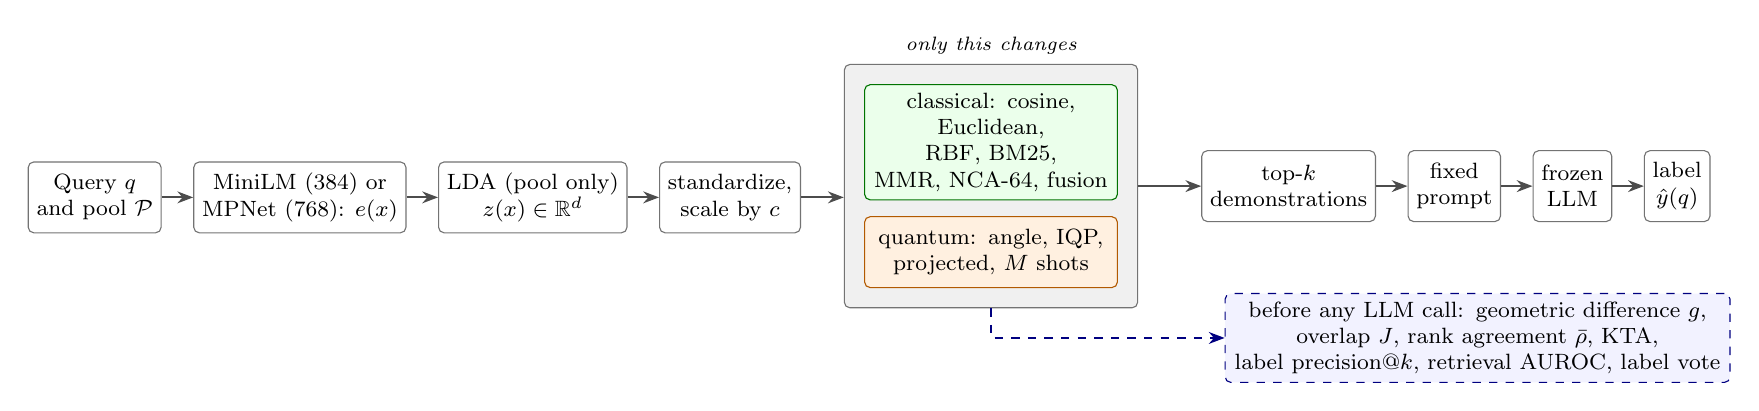
\begin{tikzpicture}[
  font=\footnotesize, node distance=4.5mm and 4mm,
  box/.style={draw=black!55, rounded corners=2pt, align=center, inner sep=3pt, minimum height=9mm, fill=white},
  sel/.style={box, fill=black!6},
  q/.style={box, fill=orange!12, draw=orange!70!black},
  c/.style={box, fill=green!8, draw=green!45!black},
  diag/.style={box, fill=blue!5, draw=blue!50!black, dashed},
  arr/.style={-{Stealth[length=2mm]}, thick, black!70}]
\node[box] (txt) {Query $q$\\and pool $\mathcal{P}$};
\node[box, right=of txt] (emb) {MiniLM (384) or\\MPNet (768): $e(x)$};
\node[box, right=of emb] (lda) {LDA (pool only)\\$z(x)\in\mathbb{R}^{d}$};
\node[box, right=of lda] (std) {standardize,\\scale by $c$};
\node[c, right=8mm of std, yshift=7mm, text width=30mm] (ck) {classical: cosine,\\Euclidean, RBF, BM25,\\MMR, NCA-64, fusion};
\node[q, below=2mm of ck, text width=30mm] (qk) {quantum: angle, IQP,\\projected, $M$ shots};
\begin{scope}[on background layer]
\node[sel, fit=(ck)(qk), inner sep=2.5mm, label={[font=\scriptsize\itshape]above:only this changes}] (selbox) {};
\end{scope}
\node[box, right=8mm of selbox] (topk) {top-$k$\\demonstrations};
\node[box, right=of topk] (prm) {fixed\\prompt};
\node[box, right=of prm] (llm) {frozen\\LLM};
\node[box, right=of llm] (out) {label\\$\hat y(q)$};
\draw[arr] (txt) -- (emb); \draw[arr] (emb) -- (lda); \draw[arr] (lda) -- (std);
\draw[arr] (std) -- (selbox.west|-std); \draw[arr] (selbox.east|-topk) -- (topk);
\draw[arr] (topk) -- (prm); \draw[arr] (prm) -- (llm); \draw[arr] (llm) -- (out);
\node[diag, below=9mm of topk, xshift=24mm, text width=62mm] (dg) {before any LLM call: geometric difference $g$,\\overlap $J$, rank agreement $\bar\rho$, KTA,\\label precision@$k$, retrieval AUROC, label vote};
\draw[arr, dashed, blue!50!black] (selbox.south) |- (dg.west);
\end{tikzpicture}
.
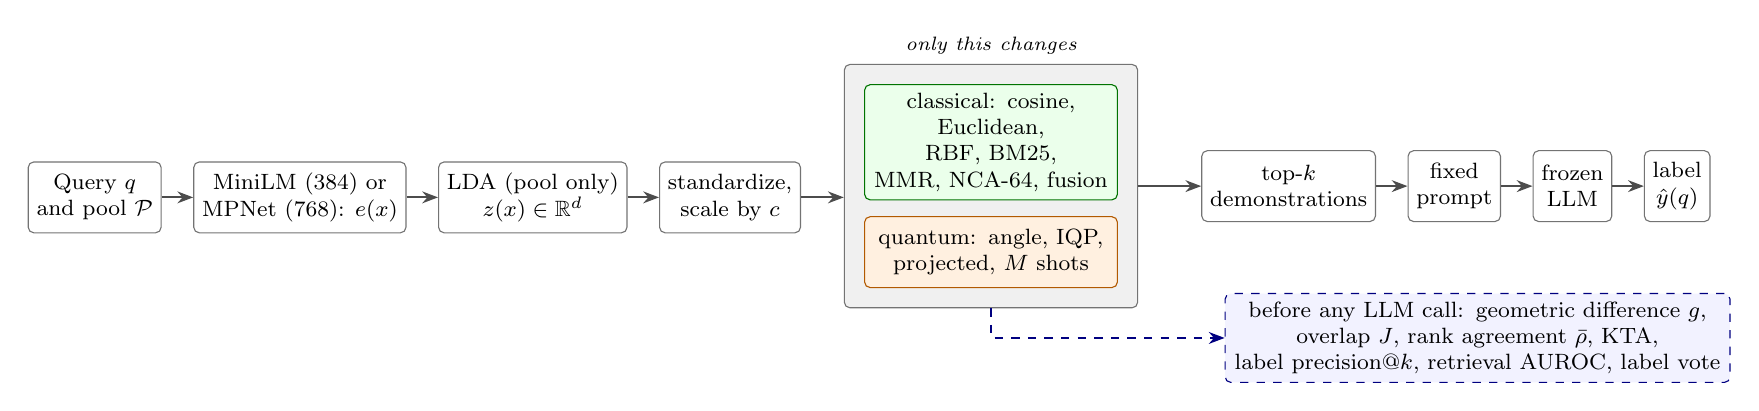
\begin{tikzpicture}[
  font=\footnotesize, node distance=4.5mm and 4mm,
  box/.style={draw=black!55, rounded corners=2pt, align=center, inner sep=3pt, minimum height=9mm, fill=white},
  sel/.style={box, fill=black!6},
  q/.style={box, fill=orange!12, draw=orange!70!black},
  c/.style={box, fill=green!8, draw=green!45!black},
  diag/.style={box, fill=blue!5, draw=blue!50!black, dashed},
  arr/.style={-{Stealth[length=2mm]}, thick, black!70}]
\node[box] (txt) {Query $q$\\and pool $\mathcal{P}$};
\node[box, right=of txt] (emb) {MiniLM (384) or\\MPNet (768): $e(x)$};
\node[box, right=of emb] (lda) {LDA (pool only)\\$z(x)\in\mathbb{R}^{d}$};
\node[box, right=of lda] (std) {standardize,\\scale by $c$};
\node[c, right=8mm of std, yshift=7mm, text width=30mm] (ck) {classical: cosine,\\Euclidean, RBF, BM25,\\MMR, NCA-64, fusion};
\node[q, below=2mm of ck, text width=30mm] (qk) {quantum: angle, IQP,\\projected, $M$ shots};
\begin{scope}[on background layer]
\node[sel, fit=(ck)(qk), inner sep=2.5mm, label={[font=\scriptsize\itshape]above:only this changes}] (selbox) {};
\end{scope}
\node[box, right=8mm of selbox] (topk) {top-$k$\\demonstrations};
\node[box, right=of topk] (prm) {fixed\\prompt};
\node[box, right=of prm] (llm) {frozen\\LLM};
\node[box, right=of llm] (out) {label\\$\hat y(q)$};
\draw[arr] (txt) -- (emb); \draw[arr] (emb) -- (lda); \draw[arr] (lda) -- (std);
\draw[arr] (std) -- (selbox.west|-std); \draw[arr] (selbox.east|-topk) -- (topk);
\draw[arr] (topk) -- (prm); \draw[arr] (prm) -- (llm); \draw[arr] (llm) -- (out);
\node[diag, below=9mm of topk, xshift=24mm, text width=62mm] (dg) {before any LLM call: geometric difference $g$,\\overlap $J$, rank agreement $\bar\rho$, KTA,\\label precision@$k$, retrieval AUROC, label vote};
\draw[arr, dashed, blue!50!black] (selbox.south) |- (dg.west);
\end{tikzpicture}
.
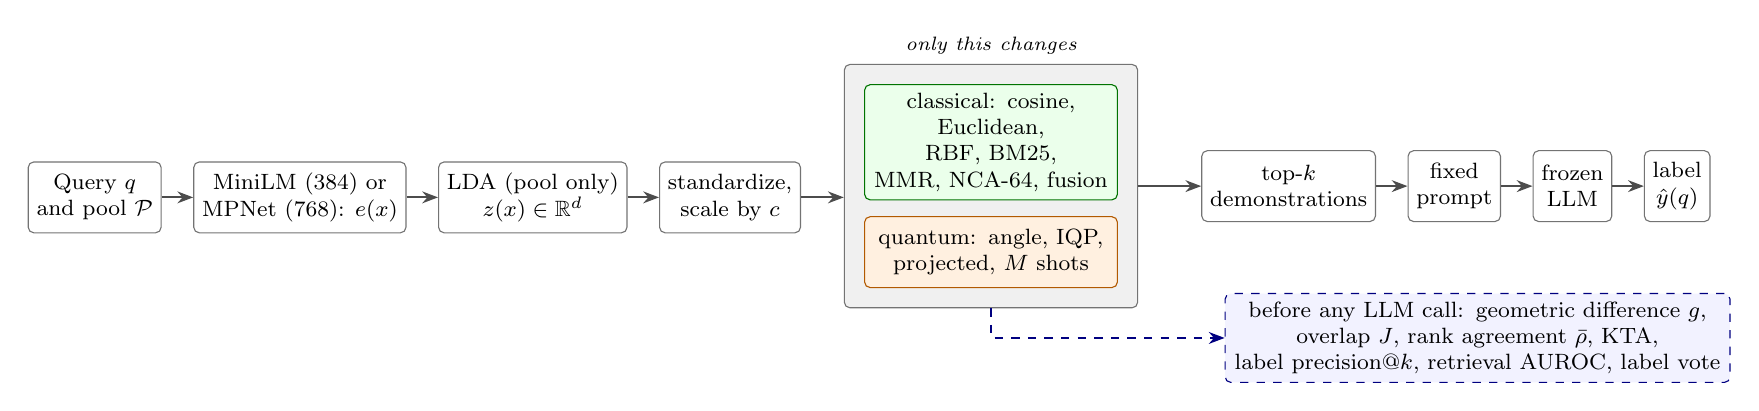
\begin{tikzpicture}[
  font=\footnotesize, node distance=4.5mm and 4mm,
  box/.style={draw=black!55, rounded corners=2pt, align=center, inner sep=3pt, minimum height=9mm, fill=white},
  sel/.style={box, fill=black!6},
  q/.style={box, fill=orange!12, draw=orange!70!black},
  c/.style={box, fill=green!8, draw=green!45!black},
  diag/.style={box, fill=blue!5, draw=blue!50!black, dashed},
  arr/.style={-{Stealth[length=2mm]}, thick, black!70}]
\node[box] (txt) {Query $q$\\and pool $\mathcal{P}$};
\node[box, right=of txt] (emb) {MiniLM (384) or\\MPNet (768): $e(x)$};
\node[box, right=of emb] (lda) {LDA (pool only)\\$z(x)\in\mathbb{R}^{d}$};
\node[box, right=of lda] (std) {standardize,\\scale by $c$};
\node[c, right=8mm of std, yshift=7mm, text width=30mm] (ck) {classical: cosine,\\Euclidean, RBF, BM25,\\MMR, NCA-64, fusion};
\node[q, below=2mm of ck, text width=30mm] (qk) {quantum: angle, IQP,\\projected, $M$ shots};
\begin{scope}[on background layer]
\node[sel, fit=(ck)(qk), inner sep=2.5mm, label={[font=\scriptsize\itshape]above:only this changes}] (selbox) {};
\end{scope}
\node[box, right=8mm of selbox] (topk) {top-$k$\\demonstrations};
\node[box, right=of topk] (prm) {fixed\\prompt};
\node[box, right=of prm] (llm) {frozen\\LLM};
\node[box, right=of llm] (out) {label\\$\hat y(q)$};
\draw[arr] (txt) -- (emb); \draw[arr] (emb) -- (lda); \draw[arr] (lda) -- (std);
\draw[arr] (std) -- (selbox.west|-std); \draw[arr] (selbox.east|-topk) -- (topk);
\draw[arr] (topk) -- (prm); \draw[arr] (prm) -- (llm); \draw[arr] (llm) -- (out);
\node[diag, below=9mm of topk, xshift=24mm, text width=62mm] (dg) {before any LLM call: geometric difference $g$,\\overlap $J$, rank agreement $\bar\rho$, KTA,\\label precision@$k$, retrieval AUROC, label vote};
\draw[arr, dashed, blue!50!black] (selbox.south) |- (dg.west);
\end{tikzpicture}
}
\caption{Pipeline. Only the selector (gray box) changes; the pool, features, prompt template, LLM and
decoding are shared. The diagnostics (dashed box) need no LLM calls and are computed before the paid
runs.}
\label{fig:pipeline}
\end{figure*}

\subsection{Problem setup}
Let $\mathcal{P}=\{(x_i,y_i)\}_{i=1}^{N}$ be a labelled pool with $N=500$ and labels from a set
$\mathcal{Y}$. For a test input $q$, a selector assigns a score $s(q,x_i)$ to every pool item and keeps
the $k$ highest, $A_k(q)$. A fixed template turns $A_k(q)$ and $q$ into a prompt, and a frozen LLM
returns a label $\hat y(q)$. Selectors differ only in how they build $A_k(q)$ (Fig.~\ref{fig:pipeline}).

\subsection{Representation}
Each text is embedded with the sentence encoder all-MiniLM-L6-v2 \cite{reimers2019sentence,wang2020minilm}
and normalized to unit length, $e(x)\in\R^{384}$; a robustness run uses all-mpnet-base-v2
\cite{song2020mpnet} ($e(x)\in\R^{768}$). Because every feature later becomes one qubit, we compress
$e(x)$ with linear discriminant analysis (LDA) \cite{fisher1936use} fitted on the pool only,
$z(x)=W^\top e(x)\in\R^{d}$. LDA yields at most $|\mathcal{Y}|-1$ directions, five for the six-class tasks,
so we use $d\in\{2,3,4,5\}$ on all datasets. Neighbourhood components analysis (NCA)
\cite{goldberger2004nca}, also fitted on the pool only, has no such cap and supplies $d\in\{6,8,10,12\}$
for the LLM runs with more qubits and the scaling study. Unlike LDA, NCA does not reduce the classes to
their means, so it leaves the kernels more room to disagree. For the RBF and quantum kernels each
feature is standardized with the pool mean and standard deviation, giving $\tilde z(x)$; the quantum
circuits receive $c\,\tilde z(x)$ for a bandwidth $c$.

\subsection{Selectors}
Table~\ref{tab:selectors} lists the selectors. S2 is standard practice \cite{liu2022makes}. S3 to S9
see the same $d$ LDA features (S5 to S9 in standardized form), so differences among them come from the
similarity function alone. The second group tests whether the quantum kernel competes with retrievers a
practitioner would actually use. S10 is BM25 on the raw text ($k_1=1.5$, $b=0.75$)
\cite{robertson2009bm25}. S11 and S12 apply MMR \cite{carbonell1998mmr}, which adds the next example
$x$ maximizing $\lambda s(q,x)-(1-\lambda)\max_{x'\in A}s(x,x')$, with $\lambda=0.5$ fixed in advance, to
the cosine and IQP kernels respectively. S13 is a trained metric retriever: NCA fitted on the pool labels
of the full embedding to 64 dimensions, ranked by Euclidean distance. S15 fuses the cosine and IQP
rankings by reciprocal rank fusion, $s=\sum_r 1/(60+\mathrm{rank}_r)$ \cite{cormack2009rrf}, and asks
whether the quantum ranking can \emph{add} to the standard one. S14 is not a selector but an upper
bound: it takes the $k$ most similar (cosine) pool items that carry the query's gold label. The gap
between S14 and the best real selector is the headroom left for any similarity function.

S16 and S17 answer the objection that a fixed quantum kernel is a straw man. Both learn one scale per
input feature, $w\in\R^d_{>0}$: S16 is the IQP kernel on $w\odot\tilde z$, and S17 is the RBF kernel
$\exp(-\sum_j w_j^2(\tilde z_j-\tilde z'_j)^2)$ with automatic relevance determination. Both maximize the
centred kernel-target alignment \cite{cortes2012centered} on 250 pool items with L-BFGS (at most 60
iterations, scales in $[10^{-3},10]$), starting from the tuned $c$ (S16) and the median-rule $\gamma$
(S17). They use the same data, objective, optimizer and parameter count, so S16 against S17 compares the
two families at their best on equal terms, in the spirit of trained quantum embedding kernels
\cite{hubregtsen2022training}.

\begin{table}[t]
\centering
\caption{Selectors. All use the same pool, prompt and LLM. S14 uses the gold label and only bounds what
selection can gain.}
\label{tab:selectors}
\footnotesize
\setlength{\tabcolsep}{3pt}
\begin{tabular}{@{}lll@{}}
\toprule
ID & Selector & Score or rule \\
\midrule
S1 & Random & uniform random (fixed seed) \\
S2 & Cosine, full embedding & $\cos(e(q),e(x))$ \\
S3 & Cosine, LDA & $\cos(z(q),z(x))$ \\
S4 & Euclidean, LDA & $-\lVert z(q)-z(x)\rVert$ \\
S5 & RBF, LDA & $\exp(-\gamma\lVert \tilde z(q)-\tilde z(x)\rVert^2)$ \\
S6 & Quantum angle & $K_A$, Eq.~\eqref{eq:closed} (control) \\
S7 & Quantum IQP & $K_B$, Eqs.~\eqref{eq:fid}, \eqref{eq:iqp} \\
S8 & Quantum projected & $K_P$, Eq.~\eqref{eq:proj} \\
S9 & Quantum IQP, $M$ shots & $\hat K_B$, Eq.~\eqref{eq:shots} (robustness) \\
\midrule
S10 & BM25 & lexical score on raw text \\
S11 & MMR, cosine & S2 relevance, $\lambda=0.5$ \\
S12 & MMR, quantum IQP & S7 relevance, $\lambda=0.5$ \\
S13 & NCA-64 & trained metric on $e(x)$ \\
S14 & Label oracle & gold-label neighbours (bound) \\
S15 & Fusion & RRF of S2 and S7 \\
\midrule
S16 & Quantum IQP, trained & $K_B$ on $w\odot\tilde z$, $w$ trained \\
S17 & RBF, trained & ARD-RBF, $w$ trained \\
\bottomrule
\end{tabular}
\end{table}

\subsection{Quantum kernels}
In this subsection $x\in\R^d$ denotes the encoded vector $c\,\tilde z(\cdot)$ of a text. A feature
map $U(x)$ on $d$ qubits prepares $\ket{\psi(x)}=U(x)\ket{0}^{\otimes d}$. The fidelity kernel is
\begin{equation}
K(x,x') = \bigl|\langle\psi(x)|\psi(x')\rangle\bigr|^2 .
\label{eq:fid}
\end{equation}

\emph{Map A (angle encoding).} $U_A(x)=\bigotimes_{j=1}^{d}R_Y(x_j)$ rotates each qubit independently
and creates no entanglement. It is widely used in hybrid NLP models \cite{vats2025survey}.

\begin{proposition}
\label{prop:angle}
For Map A, the fidelity kernel equals
\begin{equation}
K_A(x,x') = \prod_{j=1}^{d}\cos^2\!\Bigl(\frac{x_j-x'_j}{2}\Bigr),
\label{eq:closed}
\end{equation}
a product of shifted cosine kernels that a classical computer evaluates in $O(d)$ time.
\end{proposition}
\begin{paperproof}
The state is a product, $\ket{\psi_A(x)}=\bigotimes_j(\cos\frac{x_j}{2}\ket0+\sin\frac{x_j}{2}\ket1)$, so the
overlap factorizes into $\prod_j(\cos\frac{x_j}{2}\cos\frac{x'_j}{2}+\sin\frac{x_j}{2}\sin\frac{x'_j}{2})
=\prod_j\cos\frac{x_j-x'_j}{2}$. Squaring gives \eqref{eq:closed}.
\end{paperproof}

The observation is known and elementary; we state it for completeness because it matters for
interpretation: anything obtained with Map A is a classical result. Our unit tests check
\eqref{eq:closed} against the simulated circuit to $10^{-9}$.

\emph{Map B (IQP encoding).} In the spirit of Havl\'{\i}\v{c}ek et al.~\cite{havlicek2019supervised} and the
instantaneous quantum polynomial circuits of \cite{shepherd2009temporally}, we use the
\texttt{IQPEmbedding} of PennyLane, whose pair terms use $x_jx_l$ instead of the
$(\pi-x_j)(\pi-x_l)$ of \cite{havlicek2019supervised}:
\begin{equation}
\begin{aligned}
U_B(x)&=\bigl[U_Z(x)\,H^{\otimes d}\bigr]^{2},\\
U_Z(x)&=\prod_{j}R_Z(x_j)\prod_{j<l}R_{ZZ}(x_jx_l),
\end{aligned}
\label{eq:iqp}
\end{equation}
with $R_Z(\theta)=e^{-i\theta Z/2}$ and $R_{ZZ}(\theta)=e^{-i\theta Z_jZ_l/2}$ on every pair of qubits
(Fig.~\ref{fig:circuits}). The pairwise terms entangle the register, and the resulting kernel $K_B$ has
no known product form.

\emph{Projected kernel.} To reduce concentration, Huang et al.~\cite{huang2021power} compare the
one-qubit reduced states $\rho_j(x)$ instead of the full state. We use their Bloch vectors
$b_j(x)=(\langle X_j\rangle,\langle Y_j\rangle,\langle Z_j\rangle)$ from Map B and define
\begin{equation}
K_P(x,x')=\exp\Bigl(-\gamma_P\sum_{j=1}^{d}\lVert b_j(x)-b_j(x')\rVert^2\Bigr).
\label{eq:proj}
\end{equation}
Since $\lVert\rho_j-\rho'_j\rVert_F^2=\tfrac12\lVert b_j-b'_j\rVert^2$, this matches their definition up
to a constant absorbed in $\gamma_P$.

\emph{Finite shots.} On hardware, $K_B(x,x')$ is the probability of reading all zeros after
$U_B(x')^\dagger U_B(x)$ (Fig.~\ref{fig:circuits}c). With $M$ shots the estimate is binomial,
\begin{equation}
\hat K_B(x,x') = B/M,\qquad B\sim\mathrm{Binomial}\bigl(M,K_B(x,x')\bigr),
\label{eq:shots}
\end{equation}
and S9 uses $M=1{,}024$. It models shot noise only; gate noise is treated in Section~\ref{sec:noise}.

\begin{figure}[t]
\centering
% Circuit figure (quantikz). Used by main.tex as % Circuit figure (quantikz). Used by main.tex as % Circuit figure (quantikz). Used by main.tex as \input{fig_circuits}.
\footnotesize
\begin{tabular}{@{}c@{\hspace{3mm}}c@{}}
(a) Map A & (b) one layer of Map B \\[1mm]
\begin{quantikz}[row sep=0.12cm, column sep=0.18cm]
\lstick{$\ket{0}$} & \gate{R_Y(x_1)} & \qw \\
\lstick{$\ket{0}$} & \gate{R_Y(x_2)} & \qw \\
\lstick{$\ket{0}$} & \gate{R_Y(x_3)} & \qw
\end{quantikz}
&
\begin{quantikz}[row sep=0.12cm, column sep=0.18cm]
\lstick{$\ket{0}$} & \gate{H} & \gate{R_Z(x_1)} & \gate[3]{\displaystyle\prod_{j<l}R_{ZZ}(x_jx_l)} & \qw \\
\lstick{$\ket{0}$} & \gate{H} & \gate{R_Z(x_2)} & & \qw \\
\lstick{$\ket{0}$} & \gate{H} & \gate{R_Z(x_3)} & & \qw
\end{quantikz}
\\[2mm]
\multicolumn{2}{c}{(c) kernel estimation: $K(x,x')=\Pr[\,000\,]$} \\[1mm]
\multicolumn{2}{c}{
\begin{quantikz}[row sep=0.12cm, column sep=0.25cm]
\lstick{$\ket{0}$} & \gate[3]{U(x)} & \gate[3]{U(x')^{\dagger}} & \meter{} \\
\lstick{$\ket{0}$} & & & \meter{} \\
\lstick{$\ket{0}$} & & & \meter{}
\end{quantikz}}
\end{tabular}
.
\footnotesize
\begin{tabular}{@{}c@{\hspace{3mm}}c@{}}
(a) Map A & (b) one layer of Map B \\[1mm]
\begin{quantikz}[row sep=0.12cm, column sep=0.18cm]
\lstick{$\ket{0}$} & \gate{R_Y(x_1)} & \qw \\
\lstick{$\ket{0}$} & \gate{R_Y(x_2)} & \qw \\
\lstick{$\ket{0}$} & \gate{R_Y(x_3)} & \qw
\end{quantikz}
&
\begin{quantikz}[row sep=0.12cm, column sep=0.18cm]
\lstick{$\ket{0}$} & \gate{H} & \gate{R_Z(x_1)} & \gate[3]{\displaystyle\prod_{j<l}R_{ZZ}(x_jx_l)} & \qw \\
\lstick{$\ket{0}$} & \gate{H} & \gate{R_Z(x_2)} & & \qw \\
\lstick{$\ket{0}$} & \gate{H} & \gate{R_Z(x_3)} & & \qw
\end{quantikz}
\\[2mm]
\multicolumn{2}{c}{(c) kernel estimation: $K(x,x')=\Pr[\,000\,]$} \\[1mm]
\multicolumn{2}{c}{
\begin{quantikz}[row sep=0.12cm, column sep=0.25cm]
\lstick{$\ket{0}$} & \gate[3]{U(x)} & \gate[3]{U(x')^{\dagger}} & \meter{} \\
\lstick{$\ket{0}$} & & & \meter{} \\
\lstick{$\ket{0}$} & & & \meter{}
\end{quantikz}}
\end{tabular}
.
\footnotesize
\begin{tabular}{@{}c@{\hspace{3mm}}c@{}}
(a) Map A & (b) one layer of Map B \\[1mm]
\begin{quantikz}[row sep=0.12cm, column sep=0.18cm]
\lstick{$\ket{0}$} & \gate{R_Y(x_1)} & \qw \\
\lstick{$\ket{0}$} & \gate{R_Y(x_2)} & \qw \\
\lstick{$\ket{0}$} & \gate{R_Y(x_3)} & \qw
\end{quantikz}
&
\begin{quantikz}[row sep=0.12cm, column sep=0.18cm]
\lstick{$\ket{0}$} & \gate{H} & \gate{R_Z(x_1)} & \gate[3]{\displaystyle\prod_{j<l}R_{ZZ}(x_jx_l)} & \qw \\
\lstick{$\ket{0}$} & \gate{H} & \gate{R_Z(x_2)} & & \qw \\
\lstick{$\ket{0}$} & \gate{H} & \gate{R_Z(x_3)} & & \qw
\end{quantikz}
\\[2mm]
\multicolumn{2}{c}{(c) kernel estimation: $K(x,x')=\Pr[\,000\,]$} \\[1mm]
\multicolumn{2}{c}{
\begin{quantikz}[row sep=0.12cm, column sep=0.25cm]
\lstick{$\ket{0}$} & \gate[3]{U(x)} & \gate[3]{U(x')^{\dagger}} & \meter{} \\
\lstick{$\ket{0}$} & & & \meter{} \\
\lstick{$\ket{0}$} & & & \meter{}
\end{quantikz}}
\end{tabular}

\caption{Circuits for $d=3$. (a) Map A, no entangling gates. (b) One layer of Map B; the layer is
applied twice. (c) Kernel estimation on hardware: the probability of the all-zero outcome equals
$K(x,x')$.}
\label{fig:circuits}
\end{figure}

\subsection{What retrieval can see of a kernel}
\label{sec:rank}
A selector keeps the $k$ highest scores of each query and discards the values. This simple fact shapes
the whole study.

\begin{proposition}
\label{prop:rank}
Let $f_q:\R\to\R$ be strictly increasing for every query $q$. The scores $s(q,x)$ and $f_q(s(q,x))$
retrieve the same set $A_k(q)$ for every $q$ (with the same tie-breaking). In particular: (a) the RBF
kernel retrieves the same items for every $\gamma>0$; (b) for fixed $c$, the projected kernel retrieves
the same items for every $\gamma_P>0$; (c) global depolarizing noise of any strength $p<1$ applied to the
encoded states, $\rho\mapsto(1-p)\rho+p\,I/2^d$, does not change the items retrieved by the fidelity
kernel.
\end{proposition}
\begin{paperproof}
A strictly increasing map preserves the order of each row of scores, and $A_k(q)$ depends on that order
only. (a) $e^{-\gamma u}$ is decreasing in the squared distance $u$ for any $\gamma>0$, so every $\gamma$
induces the same order. (b) is the same argument on Bloch-vector distances. (c) For noisy states the
swap test measures $\Tr(\tilde\rho\tilde\rho')=(1-p)^2K+\bigl(1-(1-p)^2\bigr)/2^d$, and the
compute-uncompute circuit with a final global channel gives $(1-p)K+p/2^d$; both are affine in $K$
with positive slope.
\end{paperproof}

The proposition covers selectors that rank one score per item. MMR (S11, S12) mixes kernel values, so
it is invariant only under positive affine maps, which still include case (c). Three consequences follow. The RBF and projected bandwidths need no tuning for retrieval; they affect
only diagnostics computed from kernel values. Hardware noise can only harm a quantum selector through
noise that is \emph{not} a global affine map of the kernel: local gate errors, which act differently on
different inputs, and finite sampling. And the geometric difference $g$ \cite{huang2021power}, designed
for kernel regression, is not invariant under such transforms, so it can report a difference that
retrieval never sees. We therefore add a diagnostic that is: the \emph{rank agreement}
$\bar\rho(K,K')=\frac{1}{|Q|}\sum_q\mathrm{Spearman}\bigl(K(q,\cdot),K'(q,\cdot)\bigr)$, the mean per-query
rank correlation of two kernels over the pool. Two selectors with $\bar\rho$ close to one build nearly the
same prompts whatever their values look like.

\subsection{Tuning}
\label{sec:tune}
Quantum kernels are sensitive to input scaling \cite{shaydulin2022importance,canatar2023bandwidth}, so
we tune the bandwidth $c\in\{0.1,0.25,0.5,1\}$ once per seed and dimension. The criterion is the
accuracy of a $k$-nearest-neighbour vote with the IQP kernel on a validation set of 100 training items
disjoint from the pool; ties go to the smaller value, and S6 to S9 and S12 share the chosen $c$. Neither the
LLM nor any test item is involved. By Proposition~\ref{prop:rank} the classical kernels need no
counterpart. The RBF parameter matters only for $g$, where we give the classical side the benefit of
the doubt and report the smallest $g$ over $\gamma=m\gamma_0$, $m\in\{0.25,0.5,1,2\}$, with $\gamma_0$ the
inverse median squared pairwise distance on the pool ($\gamma_P$ uses the same median rule on Bloch
vectors). If anything, this protocol favours the quantum side, which gets four validated candidates for
its only parameter that changes retrieval. Because the vote is only a proxy for what the LLM needs, a
separate study (Section~\ref{sec:bw}) re-tunes $c$ with the LLM itself.

\subsection{Prompting and inference}
Every selector uses one template per dataset: a one-line instruction listing the label words, the $k$
demonstrations as ``Question:/Answer:'' pairs (``Text:'' for Emotion and DBpedia-14, ``Query:'' for
Banking77), and the query.
Demonstrations are printed from least to most similar, so the nearest one sits directly above the query
(MMR keeps its selection order, most relevant last). We decode greedily with at most 24 new tokens,
keep the first line of the reply, lowercase it and strip surrounding punctuation; spaces and hyphens may
also be read as underscores (Banking77 intent names). A reply counts as a label if it equals it, if it
starts with it followed by a non-letter (the longest such label wins), or, when at least ten characters
long, if it is a prefix of exactly one label (a name cut off by the token limit); anything else counts as
wrong. Answers are cached by the exact prompt, so two selectors that pick
the same demonstrations in the same order receive the same answer.

We use three LLMs. The main model is \TModelName{}, queried through its API at temperature 0. The second
is Qwen2.5-1.5B-Instruct \cite{qwen2025qwen25}, an open-weight model run locally, and the third is
Qwen2.5-7B-Instruct, run locally with 4-bit NF4 quantization \cite{dettmers2023qlora}. For the 1.5B model we also
compute a probability for every label (seed 0, datasets with at most 20 labels),
$p(y\mid\text{prompt})\propto\sum_{v\in V(y)}\exp\log p(v\mid\text{prompt})$, where $V(y)$ holds the
lower-case and capitalized spellings of the label word and $\log p(v\mid\cdot)$ sums the token
log-probabilities. These probabilities give LLM-level AUROC and calibration.

\subsection{Diagnostics before the LLM}
\label{sec:diag}
\emph{Overlap.} The mean Jaccard index between the sets retrieved by two selectors,
$J(A,B)=\frac{1}{|Q|}\sum_{q}|A_k(q)\cap B_k(q)|/|A_k(q)\cup B_k(q)|$.
With $J\approx1$ two selectors build nearly identical prompts.

\emph{Geometric difference.} Following Huang et al.~\cite{huang2021power}, with both pool Gram
matrices scaled to trace $N$,
\begin{equation}
g(K_C\,\|\,K_Q)=\sqrt{\lambda_{\max}\!\bigl(K_Q^{1/2}(K_C+\lambda I)^{-1}K_Q^{1/2}\bigr)},
\label{eq:g}
\end{equation}
with $\lambda=10^{-3}$. Values near one mean that the classical kernel $K_C$ can already express what
the quantum kernel $K_Q$ expresses on this pool. Besides RBF we use the cosine kernel
$\cos^2$ on LDA features (positive semidefinite) as $K_C$.

\emph{Rank agreement} $\bar\rho$, defined in Section~\ref{sec:rank}, and \emph{kernel-target alignment}
\cite{cristianini2002kta}, $\mathrm{KTA}(K)=\langle K,Y\rangle_F/(\lVert K\rVert_F\lVert Y\rVert_F)$
with $Y_{ij}=\mathbb{1}[y_i=y_j]$, computed on the pool Gram matrix as in the original definition.
KTA measures how well a kernel's geometry matches the labels without any learner; like $g$, it depends
on kernel values and is not invariant under the transforms of Proposition~\ref{prop:rank}. For RBF it uses
the $\gamma$ that gives the smallest $g$ (Section~\ref{sec:tune}); in the scaling study, the median rule $\gamma_0$.
On the LDA settings, rank agreement is computed on the 100 validation queries; in the scaling study, on
the test queries. The table of geometric differences reports $g$ both at the minimizing $\gamma$ and at the
median rule $\gamma_0$, since the minimum favours the conclusion that the kernels do not differ.

\emph{Label precision.} $\mathrm{Prec}@k(q)=\frac1k\sum_{x_i\in A_k(q)}\mathbb{1}[y_i=y(q)]$, the share of
retrieved demonstrations that carry the query's true label.

\emph{Retrieval AUROC.} For each query, the probability that a random same-label pool item is scored
above a random different-label item (ties count one half),
\begin{equation}
\mathrm{AUROC}_\mathrm{ret}(q)=\Pr\bigl[s(q,x^+)>s(q,x^-)\bigr],
\label{eq:auroc}
\end{equation}
averaged over queries \cite{fawcett2006roc}. Unlike precision at $k$, it reflects the full ranking.
Rule-based selectors (S11, S12, S14) produce no single score per item and have no AUROC$_\mathrm{ret}$.

\subsection{Mechanism studies}
\label{sec:studies}
\emph{Qubit scaling.} LDA caps $d$ at $|\mathcal{Y}|-1$, so the scaling study uses NCA fitted on the pool
for $d\in\{2,3,4,5,6,8,10,12\}$. For each $d$ we tune $c$ on the validation set exactly as in the main
runs and record, on the test queries, $\bar\rho$ and $J$ between IQP and RBF, the smallest $g$, the spread
(standard deviation) of off-diagonal IQP values on the pool at the tuned $c$ and at $c=1$, KTA, retrieval
AUROC and label precision. No LLM is involved.

\emph{Gate noise.}
\label{sec:noise}
For $d=5$ we simulate density matrices of Map B with local depolarizing channels
\cite{nielsen2010quantum}: after each Hadamard layer every qubit receives one-qubit noise $p_1$, and after
each phase layer every qubit receives $p_1+(d-1)p_2$, a first-order account of its one $R_Z$ and $d-1$
two-qubit gates, with $p_1=p_2/10$ and $p_2\in\{0,10^{-3},3\cdot10^{-3},10^{-2},3\cdot10^{-2}\}$. The
kernel is $\Tr(\rho\rho')$, as a swap test measures it; we use exact probabilities and $1{,}024$ swap-test
shots, where the all-zero ancilla probability is $(1+\Tr\rho\rho')/2$. As a check of
Proposition~\ref{prop:rank}(c) we also apply global depolarizing noise, which must leave every pick
unchanged.

\emph{Bandwidth with the LLM.}
\label{sec:bw}
For seed 0 and every $d$, the open 1.5B model answers the 100 validation queries and the test queries with
S7 and S8 at every candidate $c$; we choose $c$ by the validation accuracy of S7 and report the test
accuracy at every $c$, so the reader can see the IQP-minus-RBF gap under any choice. RBF needs no counterpart (Proposition~\ref{prop:rank}).

% ---------------------------------------------------------------------
\section{Experimental Setup}

\subsection{Datasets and runs}
TREC \cite{li2002learning} (6 question types, 5{,}452 training and 500 test questions) is our main
dataset. Emotion \cite{saravia2018carer} contains short, noisy tweets with six emotions. DBpedia-14
\cite{zhang2015character} has fourteen topics, more classes than qubits, which tests whether a few
qubits can separate many labels. Banking77 \cite{casanueva2020efficient} has 77 fine-grained customer
intents (10{,}003 training and 3{,}080 test queries); it is the harder task, where five supervised
features are unlikely to separate the classes and a similarity function may have more room to matter. For the three larger
datasets we draw stratified samples of at most 6{,}000 training and 500 test items; DBpedia texts are the
title plus the first 300 characters of the abstract. For every dataset and seed we draw one
label-stratified sample of 600 training items and split it at random into the pool (500) and the
validation set (100); no test item is ever used for fitting or tuning.

The main setting uses $k=4$ and $d\in\{2,3,4,5\}$ (LDA). The main LLM runs three pool seeds on TREC and
one on Emotion and DBpedia-14; the 1.5B model runs three seeds on these three datasets and seed 0 on
Banking77; the 7B model runs seed 0 at $d=5$. With seed 0 and the 1.5B model we further run NCA features
with $d\in\{6,8,10,12\}$ on all four datasets, vary $k\in\{2,4,8,16\}$, replace MiniLM by MPNet on TREC,
reorder the demonstrations, run the bandwidth study, and repeat the main setting on 2{,}000 test items for
Emotion, DBpedia-14 and Banking77 (TREC's official test set has 500 items). The main LLM additionally runs
S9 against S7 and NCA features with $d\in\{6,8\}$ on TREC.

\subsection{Metrics and statistics}
We report accuracy and macro-F1, retrieval AUROC (Eq.~\ref{eq:auroc}), label precision, and the
accuracy of a majority vote over the retrieved labels (ties go to the nearest), which shows how much the
LLM adds beyond the labels themselves. For the 1.5B model we add one-vs-rest macro AUROC
\cite{fawcett2006roc} and expected calibration error (ECE, ten bins) \cite{guo2017calibration}.

\emph{Per setting.} For each seed and dimension we compute the accuracy gap with a 95\% paired bootstrap
interval over queries (1{,}000 resamples) and an exact McNemar test \cite{mcnemar1947note}. Comparisons
fall into three preregistered families, each corrected separately with Holm's method \cite{holm1979simple}
over all its tests and settings \cite{dror2018hitchhiker}: \emph{primary}, S7 against S5 and against S3;
\emph{secondary}, S7 against the strongest classical retrievers, S2 and S13; and \emph{exploratory}, S8
against S5, S12 against S11, S15 against S2, S16 against S17 and S16 against S7. Every other analysis
(more qubits, Banking77, the larger test sets, the $k$ sweep, order, bandwidth, robustness and difficulty
strata) is exploratory, reported without correction and marked as such.

\emph{Pooled.} Each query's gap is first averaged over all its seeds and sizes, and the interval comes from a
cluster bootstrap over queries, so the same query never counts as independent evidence twice. A
non-significant difference is not evidence of no difference, so we add a two one-sided tests (TOST)
equivalence test \cite{schuirmann1987tost,lakens2017equivalence} with the preregistered margin of
$\pm\REquivMargin$ points: the gap is \emph{equivalent to zero} when the 90\% bootstrap interval lies inside
the margin ($\alpha=0.05$). We chose the margin before any LLM run as the smallest gain a practitioner
would trade a quantum circuit for: prompt format, example order and the random draw of examples move
few-shot accuracy by several points and often far more \cite{lu2022fantastically,zhao2021calibrate}, so a
smaller effect could not be acted on. \TMarginCheck{} We also report the minimum detectable effect (MDE) at 80\%
power, $(z_{0.975}+z_{0.8})\,\hat\sigma/\sqrt{n}$ over the per-query gaps, so the reader can judge what the
study could have found \cite{card2020power}; the 2{,}000-item test sets exist to bring the MDE below the
margin. Finally, we split the test queries into terciles of difficulty and report the IQP-minus-RBF gap
per tercile. Difficulty is the retrieval AUROC of cosine on the full embedding, a selector outside the
comparison; defining it by RBF itself would favour IQP on the hard tercile through regression to the mean.

\subsection{Decision rules}
Before the main run we froze the following rules in a dated file. We conclude that the quantum kernel
\emph{did better} only if (i) the interval for S7 minus S5 lies above zero and the Holm-corrected
$p<0.05$; (ii) the gap is at least 2 points; (iii) (i) and (ii) hold in at least two of three seeds
(one of one for single-seed runs) and in at least three of four dimensions; (iv) S7 beats random
selection and the LLM beats the label vote with S7; and (v) $J(\mathrm{S5},\mathrm{S7})<0.9$ and $g>1$.
Conditions (iv) use accuracies averaged over settings, and (v) must hold in every setting. Using the
same count as in (iii), we call the result \emph{no practical difference} when the whole interval lies
within $\pm2$ points, \emph{quantum worse} when it lies below zero with a gap of at least 2 points and
Holm-corrected $p<0.05$, and \emph{mixed} otherwise. A general claim requires the same verdict on at least
two of the three main datasets. The pooled TOST result is reported next to the verdict; it does not
replace it.

\subsection{Implementation}
Circuits are simulated as exact state vectors with PennyLane \cite{bergholm2018pennylane} and
cross-checked against an independent NumPy implementation, which also runs the density-matrix noise
model, the scaling study and the training of S16. Each state is computed once, so a $500\times500$
kernel needs 1{,}000 circuit evaluations. The open LLMs ran on one NVIDIA T4 GPU. \TImplementation{}

% ---------------------------------------------------------------------
\section{Results}

\subsection{Main comparison (RQ1)}

\begin{table*}[t]
\centering
\caption{LLM accuracy and macro-F1 (\%) with the main LLM, $k=4$, averaged over $d\in\{2,\dots,5\}$.
TREC shows mean$\pm$std over three seeds; the other datasets use seed 0. AUROC$_\mathrm{ret}$ is the
retrieval AUROC of Eq.~\eqref{eq:auroc} ($\times100$). Best value per column in bold.}
\label{tab:main}
\footnotesize
\begin{tabular}{@{}l ccc cc cc@{}}
\toprule
 & \multicolumn{3}{c}{TREC (3 seeds)} & \multicolumn{2}{c}{Emotion} & \multicolumn{2}{c}{DBpedia-14} \\
\cmidrule(lr){2-4}\cmidrule(lr){5-6}\cmidrule(lr){7-8}
Selector & Acc & Macro-F1 & AUROC$_\mathrm{ret}$ & Acc & Macro-F1 & Acc & Macro-F1 \\
\midrule
Zero-shot ($k{=}0$) & XYZ & XYZ & -- & -- & -- & -- & -- \\
\midrule
Random & XYZ & XYZ & XYZ & XYZ & XYZ & XYZ & XYZ \\
Cosine, 384-d & XYZ & XYZ & XYZ & XYZ & XYZ & XYZ & XYZ \\
Cosine, LDA & XYZ & XYZ & XYZ & XYZ & XYZ & XYZ & XYZ \\
Euclidean, LDA & XYZ & XYZ & XYZ & XYZ & XYZ & XYZ & XYZ \\
RBF, LDA & XYZ & XYZ & XYZ & XYZ & XYZ & XYZ & XYZ \\
\midrule
Quantum angle & XYZ & XYZ & XYZ & XYZ & XYZ & XYZ & XYZ \\
Quantum IQP & XYZ & XYZ & XYZ & XYZ & XYZ & XYZ & XYZ \\
Quantum projected & XYZ & XYZ & XYZ & XYZ & XYZ & XYZ & XYZ \\
\bottomrule
\end{tabular}

\end{table*}

Table~\ref{tab:main} lists the accuracy of the selectors that share the LDA features, with random and
full-embedding cosine for reference. On TREC, random demonstrations reached \RTrecAccRandom\% against
\RTrecAccCosFull\% for cosine on the full embedding, and zero-shot prompting reached \RTrecAccZero\%. The
quantum IQP selector reached \RTrecAccIqp\%, compared with \RTrecAccRbf\% for the RBF kernel and
\RTrecAccCosLda\% for cosine on the same LDA features. \TMainPattern{}

\begin{table}[t]
\centering
\caption{Accuracy gaps in points, pooled over seeds, dimensions and queries, with 95\% cluster bootstrap
intervals. B/E/W/U counts the settings (seed $\times$ $d$) that the per-setting rule judged better,
equivalent (95\% interval within $\pm2$ points), worse or unclear for IQP vs.\ RBF.
Verdicts follow the preregistered rules.}
\label{tab:stats}
\footnotesize
\setlength{\tabcolsep}{2.2pt}
\resizebox{\columnwidth}{!}{\begin{tabular}{@{}ll ccc cc@{}}
\toprule
Data & LLM & IQP$-$RBF & IQP$-$Cos(LDA) & Proj.$-$RBF & B/E/W/U & Verdict \\
\midrule
TREC & main LLM & XYZ XYZ & XYZ XYZ & XYZ XYZ & XYZ & XYZ \\
Emotion &  & XYZ XYZ & XYZ XYZ & XYZ XYZ & XYZ & XYZ \\
DBpedia-14 &  & XYZ XYZ & XYZ XYZ & XYZ XYZ & XYZ & XYZ \\
\midrule
TREC & Qwen2.5-1.5B & XYZ XYZ & XYZ XYZ & XYZ XYZ & XYZ & XYZ \\
Emotion &  & XYZ XYZ & XYZ XYZ & XYZ XYZ & XYZ & XYZ \\
DBpedia-14 &  & XYZ XYZ & XYZ XYZ & XYZ XYZ & XYZ & XYZ \\
\bottomrule
\end{tabular}
}
\end{table}

Table~\ref{tab:stats} gives the paired comparisons. With the main LLM, the IQP-minus-RBF gap was
\RGapTrecMain{} points on TREC (\RCITrecMain), \RGapEmotionMain{} on Emotion (\RCIEmotionMain) and
\RGapDbpediaMain{} on DBpedia-14 (\RCIDbpediaMain). The verdicts were \emph{\RVerdictTrecMain},
\emph{\RVerdictEmotionMain} and \emph{\RVerdictDbpediaMain}, respectively. With the open LLM the gaps
were \RGapTrecOpen, \RGapEmotionOpen{} and \RGapDbpediaOpen{} points. \TRqOne{}

\begin{table*}[t]
\centering
\caption{Pooled gaps (points, main LLM) for every preregistered contrast, with the TOST equivalence
$p$-value for a margin of $\pm\REquivMargin$ points ($^\ast$: equivalent at $\alpha=0.05$) and the minimum
detectable effect at 80\% power. Families are Holm-corrected separately in the per-setting tests.}
\label{tab:equiv}
\footnotesize
\setlength{\tabcolsep}{3pt}
\resizebox{\textwidth}{!}{\begin{tabular}{@{}ll ccc ccc ccc@{}}
\toprule
 & & \multicolumn{3}{c}{TREC} & \multicolumn{3}{c}{Emotion} & \multicolumn{3}{c}{DBpedia-14} \\
\cmidrule(lr){3-5}\cmidrule(lr){6-8}\cmidrule(lr){9-11}
Family & Contrast & Gap [95\% CI] & $p_\mathrm{TOST}$ & MDE & Gap [95\% CI] & $p_\mathrm{TOST}$ & MDE & Gap [95\% CI] & $p_\mathrm{TOST}$ & MDE \\
\midrule
Primary & IQP $-$ RBF & XYZ & XYZ & XYZ & XYZ & XYZ & XYZ & XYZ & XYZ & XYZ \\
Primary & IQP $-$ Cos (LDA) & XYZ & XYZ & XYZ & XYZ & XYZ & XYZ & XYZ & XYZ & XYZ \\
\midrule
Secondary & IQP $-$ Cos (384-d) & XYZ & XYZ & XYZ & XYZ & XYZ & XYZ & XYZ & XYZ & XYZ \\
Secondary & IQP $-$ NCA-64 & XYZ & XYZ & XYZ & XYZ & XYZ & XYZ & XYZ & XYZ & XYZ \\
\midrule
Exploratory & Proj. $-$ RBF & XYZ & XYZ & XYZ & XYZ & XYZ & XYZ & XYZ & XYZ & XYZ \\
Exploratory & MMR-IQP $-$ MMR-Cos & XYZ & XYZ & XYZ & XYZ & XYZ & XYZ & XYZ & XYZ & XYZ \\
Exploratory & Fusion $-$ Cos (384-d) & XYZ & XYZ & XYZ & XYZ & XYZ & XYZ & XYZ & XYZ & XYZ \\
Exploratory & Trained IQP $-$ trained RBF & XYZ & XYZ & XYZ & XYZ & XYZ & XYZ & XYZ & XYZ & XYZ \\
Exploratory & Trained IQP $-$ IQP & XYZ & XYZ & XYZ & XYZ & XYZ & XYZ & XYZ & XYZ & XYZ \\
\bottomrule
\end{tabular}
}
\end{table*}

\emph{How small is the effect?} \TEquiv{} Table~\ref{tab:equiv} gives the same quantities for every
contrast. \TRqEquiv{}

\subsection{Against stronger, diversity-aware and trained retrievers}

\begin{table}[t]
\centering
\caption{Accuracy (\%) of the classical retrievers, the quantum variants, the trained kernels and the label
oracle, averaged over $d$ and seeds, for the main LLM and the open 1.5B LLM. Best real selector per column
in bold; the last row is the oracle minus the best real selector.}
\label{tab:baselines}
\footnotesize
\setlength{\tabcolsep}{2.5pt}
\resizebox{\columnwidth}{!}{\begin{tabular}{@{}l cc cc cc@{}}
\toprule
 & \multicolumn{2}{c}{TREC} & \multicolumn{2}{c}{Emotion} & \multicolumn{2}{c}{DBpedia-14} \\
\cmidrule(lr){2-3}\cmidrule(lr){4-5}\cmidrule(lr){6-7}
Selector & Main & Open & Main & Open & Main & Open \\
\midrule
Random & XYZ & XYZ & XYZ & XYZ & XYZ & XYZ \\
BM25 (lexical) & XYZ & XYZ & XYZ & XYZ & XYZ & XYZ \\
Cosine, 384-d & XYZ & XYZ & XYZ & XYZ & XYZ & XYZ \\
MMR, cosine 384-d & XYZ & XYZ & XYZ & XYZ & XYZ & XYZ \\
NCA-64 (trained metric) & XYZ & XYZ & XYZ & XYZ & XYZ & XYZ \\
\midrule
RBF, LDA & XYZ & XYZ & XYZ & XYZ & XYZ & XYZ \\
Quantum IQP & XYZ & XYZ & XYZ & XYZ & XYZ & XYZ \\
MMR, quantum IQP & XYZ & XYZ & XYZ & XYZ & XYZ & XYZ \\
Fusion: cosine + IQP & XYZ & XYZ & XYZ & XYZ & XYZ & XYZ \\
RBF, trained scales & XYZ & XYZ & XYZ & XYZ & XYZ & XYZ \\
Quantum IQP, trained scales & XYZ & XYZ & XYZ & XYZ & XYZ & XYZ \\
\midrule
Label oracle (bound) & XYZ & XYZ & XYZ & XYZ & XYZ & XYZ \\
Headroom (oracle $-$ best) & XYZ & XYZ & XYZ & XYZ & XYZ & XYZ \\
\bottomrule
\end{tabular}
}
\end{table}

\begin{figure*}[t]
\centering
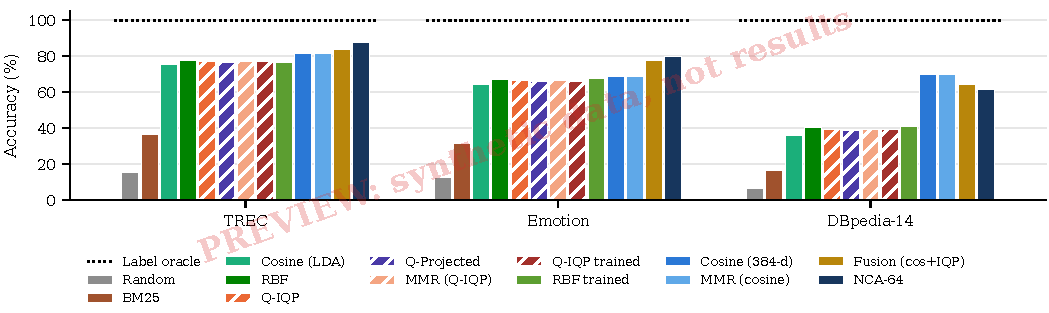
\includegraphics[width=\textwidth]{figures/fig_baselines}
\caption{Main-LLM accuracy of every selector per dataset. Hatched bars use a quantum kernel; the dotted
line is the label oracle.}
\label{fig:baselines}
\end{figure*}

A quantum kernel that only ties an RBF kernel on five features could still matter if both beat the
retrievers people use. Table~\ref{tab:baselines} and Fig.~\ref{fig:baselines} test this. \TBaselines{}
\TSecondary{} \TFusion{} The oracle row shows how much any similarity function could still gain: with
the main LLM, \RHeadroomTrecMain{} points on TREC, \RHeadroomEmotionMain{} on Emotion and
\RHeadroomDbpediaMain{} on DBpedia-14 above the best real selector.

\emph{Trained kernels.} A fixed circuit may simply be the wrong quantum kernel. When both sides learn
one input scale per feature with the same objective (S16, S17): \TTrained{}

\subsection{Why the selectors agree or differ (RQ2)}

\begin{table}[t]
\centering
\caption{Diagnostics computed without the LLM, averaged over settings. $g$: geometric difference
(Eq.~\ref{eq:g}); $J$: Jaccard overlap of retrieved sets; Prec@4: label precision; AUROC$_\mathrm{ret}$
($\times100$).}
\label{tab:diag}
\footnotesize
\setlength{\tabcolsep}{4pt}
\resizebox{\columnwidth}{!}{\begin{tabular}{@{}l ccc@{}}
\toprule
Diagnostic (no LLM) & TREC & Emotion & DBpedia-14 \\
\midrule
$g(K_\mathrm{RBF}\,\|\,K_\mathrm{IQP})$, smallest over $\gamma$ & XYZ & XYZ & XYZ \\
$g(K_\mathrm{RBF}\,\|\,K_\mathrm{IQP})$, median $\gamma_0$ & XYZ & XYZ & XYZ \\
$g(K_\mathrm{cos}\,\|\,K_\mathrm{IQP})$ & XYZ & XYZ & XYZ \\
$g(K_\mathrm{RBF}\,\|\,K_\mathrm{proj})$ & XYZ & XYZ & XYZ \\
$J$(RBF, angle) & XYZ & XYZ & XYZ \\
$J$(RBF, IQP) & XYZ & XYZ & XYZ \\
$J$(RBF, projected) & XYZ & XYZ & XYZ \\
$J$(IQP, IQP 1024 shots) & XYZ & XYZ & XYZ \\
\midrule
Precision@4, RBF & XYZ & XYZ & XYZ \\
Precision@4, IQP & XYZ & XYZ & XYZ \\
Precision@4, projected & XYZ & XYZ & XYZ \\
AUROC$_\mathrm{ret}$, RBF & XYZ & XYZ & XYZ \\
AUROC$_\mathrm{ret}$, IQP & XYZ & XYZ & XYZ \\
AUROC$_\mathrm{ret}$, cosine 384-d & XYZ & XYZ & XYZ \\
\bottomrule
\end{tabular}
}
\end{table}

Table~\ref{tab:diag} helps to read Table~\ref{tab:stats}. The overlap between RBF and the angle
kernel S6 was between \RJRbfAngleMin{} and \RJRbfAngleMax{} across datasets. A high value is expected
from Eq.~\eqref{eq:closed}: for small differences $\cos^2(u/2)=1-u^2/4+O(u^4)$, which matches
$e^{-u^2/4}$ to second order, so Map A ranks nearby points almost as a Gaussian kernel does. The overlap
between RBF and IQP ranged from \RJRbfIqpMin{} to \RJRbfIqpMax, and the geometric difference of IQP
against RBF from \RgMin{} to \RgMax{} at the minimizing $\gamma$ (\RgMedMin{} to \RgMedMax{} at the median
rule). \TDiagInterp{}

The geometric difference compares kernel values; retrieval sees only their order. The rank agreement
measures the order directly (geometry table in the supplementary material). \TGeometry{} Kernel-target
alignment (\RKtaIqpMin{}--\RKtaIqpMax{} for IQP against \RKtaRbfMin{}--\RKtaRbfMax{} for RBF) shows whether
the quantum geometry fits the labels better than the classical one.

\begin{figure*}[t]
\centering
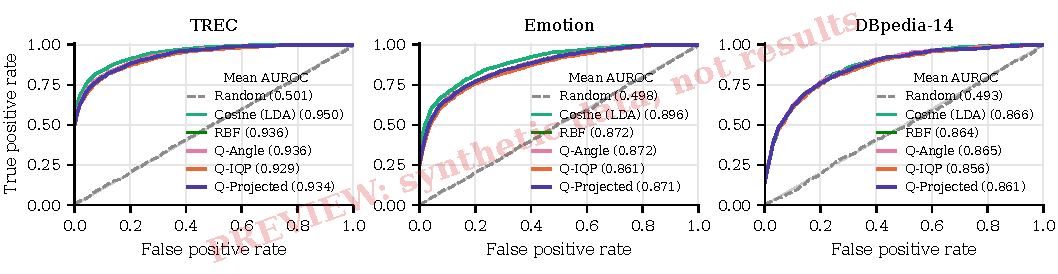
\includegraphics[width=\textwidth]{figures/fig_roc}
\caption{Retrieval ROC curves (vertically averaged over the 500 test queries) at $d=5$, seed 0. A pool
item counts as positive when it shares the query's label. Legends give the mean retrieval AUROC.}
\label{fig:roc}
\end{figure*}

Fig.~\ref{fig:roc} shows retrieval ROC curves for one setting. Averaged over all TREC settings
(Table~\ref{tab:diag}), the retrieval AUROC was \RRetIqpTrec{} for IQP and \RRetRbfTrec{} for RBF,
against \RRetCosFullTrec{} for cosine on the full embedding. \TRocComment{}

\emph{Predicting the gap before paying.} Across the \RNSettingsPbp{} TREC settings, the Spearman
correlation between the absolute IQP-minus-RBF accuracy gap and $1-J$ was \RRhoJaccard, and with $g$ it
was \RRhoG. Over all selectors, datasets and both LLMs, label precision and LLM accuracy correlated
with $\rho=$~\RRhoPrecAcc{} (supplement). \TPbp{}

\subsection{More qubits, with and without the LLM (RQ3)}

\begin{figure*}[t]
\centering
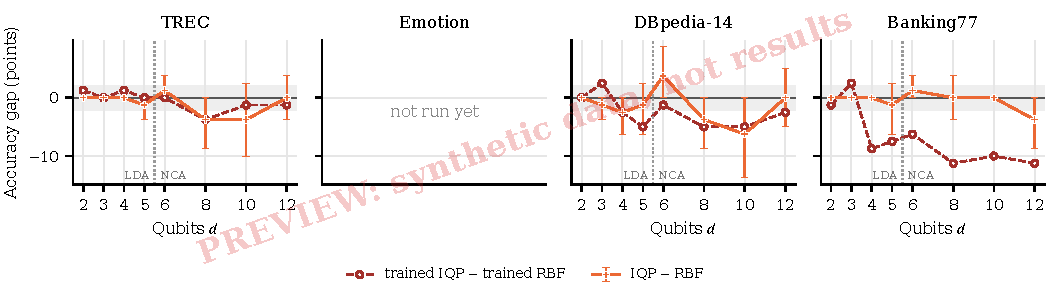
\includegraphics[width=\textwidth]{figures/fig_qubits_llm}
\caption{Exploratory. IQP-minus-RBF accuracy gap with the open 1.5B LLM from two to twelve qubits (seed 0;
LDA features up to five, NCA beyond), with 95\% bootstrap intervals; the gray band is the $\pm2$-point
margin. Dashed: the same gap for the two trained kernels.}
\label{fig:qubits_llm}
\end{figure*}

The main runs use at most five LDA features, a regime in which every distance-based kernel may find the
same neighbours. Fig.~\ref{fig:qubits_llm} lifts this limit with the LLM in the loop. \TQubits{}

\begin{figure*}[t]
\centering
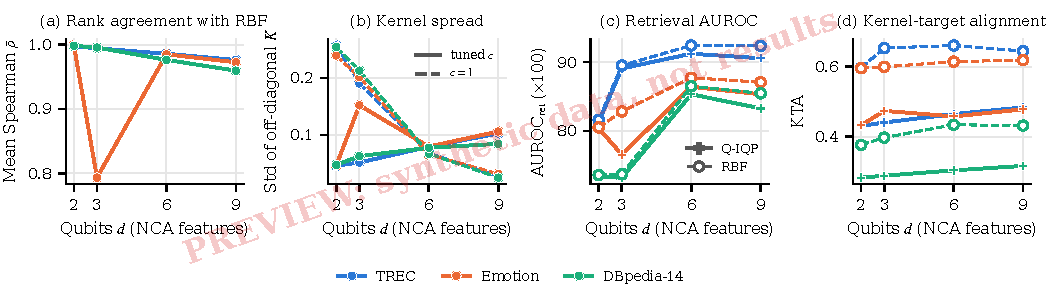
\includegraphics[width=\textwidth]{figures/fig_scaling}
\caption{Qubit scaling without the LLM (NCA features, seed 0). (a) Mean per-query rank correlation of
IQP and RBF over the pool. (b) Spread of off-diagonal IQP kernel values at the tuned bandwidth (solid)
and at $c=1$ (dashed). (c) Retrieval AUROC of IQP (solid) and RBF (dashed). (d) Kernel-target
alignment of IQP (solid) and RBF (dashed).}
\label{fig:scaling}
\end{figure*}

Fig.~\ref{fig:scaling} follows the kernels themselves from two to twelve qubits. \TScaling{}

\subsection{A harder task: Banking77}
\label{sec:banking}

\begin{table}[t]
\centering
\caption{Exploratory. Banking77 (77 intents), seed 0, averaged over $d\in\{2,\dots,5\}$: accuracy (\%)
with the open 1.5B LLM and, where run, the main LLM, and retrieval AUROC ($\times100$, open-LLM run).
Best real selector per column in bold.}
\label{tab:banking}
\footnotesize
\setlength{\tabcolsep}{4pt}
\begin{tabular}{@{}l cc c@{}}
\toprule
Selector & Acc (open) & Acc (main) & AUROC$_\mathrm{ret}$ \\
\midrule
Random & XYZ & XYZ & XYZ \\
BM25 (lexical) & XYZ & XYZ & XYZ \\
Cosine, 384-d & XYZ & XYZ & XYZ \\
MMR, cosine 384-d & XYZ & XYZ & -- \\
NCA-64 (trained metric) & XYZ & XYZ & XYZ \\
\midrule
Cosine, LDA & XYZ & XYZ & XYZ \\
RBF, LDA & XYZ & XYZ & XYZ \\
Quantum angle & XYZ & XYZ & XYZ \\
Quantum IQP & XYZ & XYZ & XYZ \\
Quantum projected & XYZ & XYZ & XYZ \\
RBF, trained scales & XYZ & XYZ & XYZ \\
Quantum IQP, trained scales & XYZ & XYZ & XYZ \\
\midrule
Label oracle (bound) & XYZ & XYZ & -- \\
\bottomrule
\end{tabular}

\end{table}

With 77 intents, a compression to five LDA features is a hard test for any similarity function, and the
label oracle shows how much room a better notion of similarity would have. \TBanking{}
Fig.~\ref{fig:qubits_llm} has a Banking77 panel with up to twelve qubits.

\subsection{Gate noise and shot noise}

\begin{figure}[t]
\centering
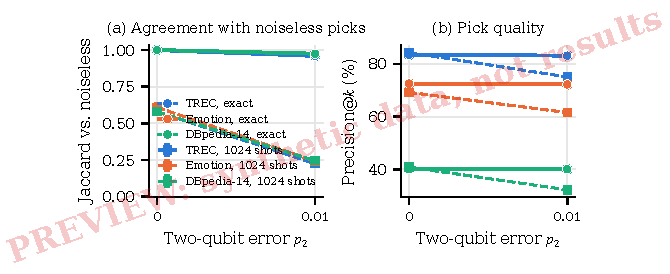
\includegraphics[width=\columnwidth]{figures/fig_noise}
\caption{Local depolarizing noise on TREC ($d=5$, seed 0). (a) Overlap of the noisy top-$k$ with the
noiseless picks, with exact probabilities (solid) and 1{,}024 swap-test shots (dashed, five draws).
(b) Label precision of the picks.}
\label{fig:noise}
\end{figure}

With 1{,}024 shots (TREC, seed 0, $d=5$), the IQP picks overlapped the exact picks with
$J=$~\RShotsJaccard, and LLM accuracy changed by \RShotsDiff{} points (\RShotsCI). Kernel concentration
and the effect of the number of shots are plotted in the supplementary material. \TShots{}
Fig.~\ref{fig:noise} adds gate noise. \TNoise{} The swap test, needed for mixed states, estimates
$(1+K)/2$ and so has a larger variance for $K$ than the compute-uncompute estimate of
Eq.~\eqref{eq:shots}; shot-only overlaps here are therefore not directly comparable with S9.
\THardware{}

\subsection{Tuning the bandwidth with the LLM}

\begin{figure}[t]
\centering
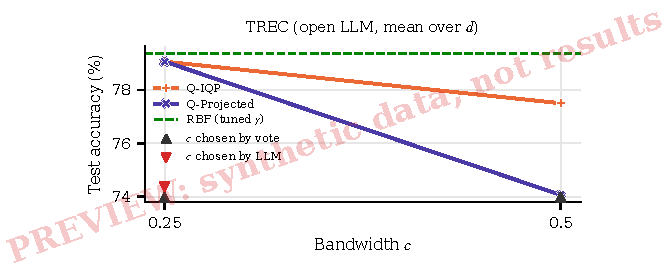
\includegraphics[width=\columnwidth]{figures/fig_bandwidth}
\caption{Exploratory. Test accuracy of the quantum selectors at every bandwidth $c$ (open 1.5B LLM, seed 0,
mean over $d$), against RBF, which does not depend on $c$. Markers at the bottom show the $c$ chosen by the
neighbour vote and by the LLM on the validation set, one per $d$.}
\label{fig:bandwidth}
\end{figure}

Our main runs tune $c$ with a neighbour vote so that the LLM never touches tuning. A reviewer may ask
whether this choice hides an advantage. Fig.~\ref{fig:bandwidth} answers it. \TBandwidth{}

\subsection{Larger LLM, another encoder, more test items and more demonstrations}

\begin{table*}[t]
\centering
\caption{Exploratory. Robustness of the IQP-minus-RBF gap (points, pooled with 95\% cluster bootstrap
intervals). Eq.: equivalent to zero within $\pm\REquivMargin$ points by TOST; the number of seeds is in
brackets. The last row uses 2{,}000 test items (not possible for TREC).}
\label{tab:robust}
\footnotesize
\setlength{\tabcolsep}{3pt}
\resizebox{\textwidth}{!}{\begin{tabular}{@{}ll cc cc cc@{}}
\toprule
 & & \multicolumn{2}{c}{TREC} & \multicolumn{2}{c}{Emotion} & \multicolumn{2}{c}{DBpedia-14} \\
\cmidrule(lr){3-4}\cmidrule(lr){5-6}\cmidrule(lr){7-8}
LLM & Encoder & IQP$-$RBF [95\% CI] & Eq.\ (seeds) & IQP$-$RBF [95\% CI] & Eq.\ (seeds) & IQP$-$RBF [95\% CI] & Eq.\ (seeds) \\
\midrule
Main LLM & MiniLM & XYZ & XYZ & XYZ & XYZ & XYZ & XYZ \\
Qwen2.5-1.5B & MiniLM & XYZ & XYZ & XYZ & XYZ & XYZ & XYZ \\
Qwen2.5-7B (4-bit) & MiniLM & XYZ & XYZ & XYZ & XYZ & XYZ & XYZ \\
Qwen2.5-1.5B & MPNet & XYZ & XYZ & XYZ & XYZ & XYZ & XYZ \\
Qwen2.5-1.5B, 2{,}000 test & MiniLM & -- & -- & XYZ & XYZ & XYZ & XYZ \\
\bottomrule
\end{tabular}
}
\end{table*}

\begin{figure*}[t]
\centering
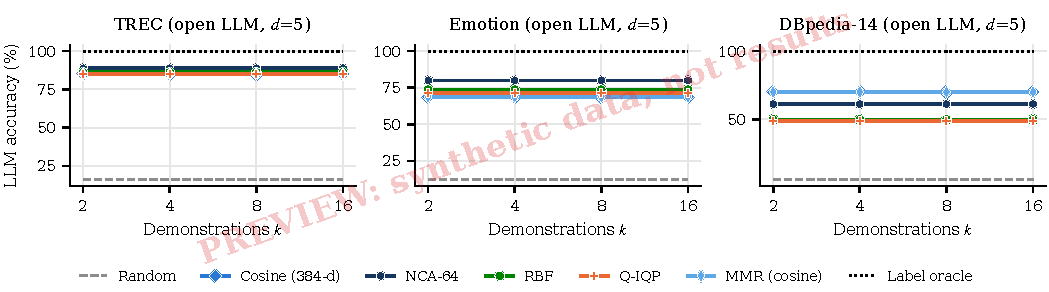
\includegraphics[width=\textwidth]{figures/fig_ksweep}
\caption{Exploratory. Accuracy against the number of demonstrations $k$ (open 1.5B LLM, seed 0, largest
$d$). The dotted line is the label oracle.}
\label{fig:ksweep}
\end{figure*}

Table~\ref{tab:robust} repeats the primary contrast with a five times larger open model (a single-seed
spot check), with a stronger encoder (TREC only), with three seeds everywhere and with four times as many
test items. \TRobust{} With 2{,}000 test items the minimum detectable effect was \RMdeLargeTestEmotion{}
points on Emotion and \RMdeLargeTestDbpedia{} on DBpedia-14 (TOST $p=$~\RTostLargeTestEmotion{} and
\RTostLargeTestDbpedia); the Banking77 result is in Section~\ref{sec:banking}. Fig.~\ref{fig:ksweep} varies the number of demonstrations. \TKSweep{}

\subsection{Difficulty, calibration, ablation and order}
These analyses are exploratory; their tables and figures are in the supplementary material.
\emph{Difficulty.} An average gap near zero could hide a kernel that helps on hard queries and hurts on
easy ones. \TDifficulty{} \emph{Calibration.} On TREC the IQP selector gave the open LLM a macro AUROC of
\ROpenTrecAurocIqp{} and an ECE of \ROpenTrecEceIqp, against \ROpenTrecAurocRbf{} and \ROpenTrecEceRbf{} for
RBF; the paired bootstrap difference in AUROC was \ROpenAurocGapTrec{} points (\ROpenAurocGapCITrec).
\TOpenCalib{} \emph{Ablation.} We changed one component of the IQP selector at a time, without the LLM.
\TAblParagraph{} \emph{Order.} Prompt order is a known source of variance \cite{lu2022fantastically}.
Keeping the retrieved sets fixed and changing only their order moved the open model's TREC accuracy by at
most \ROrderSpreadMax{} points for cosine, RBF and IQP. \TOrder{} \TErrors{}

% ---------------------------------------------------------------------
\section{Discussion}

\emph{Quantum retrieval.} A quantum kernel can only change what an LLM sees if it changes the ranking
of the pool. Our diagnostics measure this directly:
\TDiscussDiag{} \TDiscussTheory{} Proposition~\ref{prop:rank} says where any difference has to live.
Whatever distinguishes the two kernels in their values rather than in the order they give each query's
pool, or far from the query rather than among its nearest items, is thrown away by the top-$k$ rule. Near
the query, the IQP fidelity falls with a distance measured in the metric the circuit induces (its quantum
Fisher information), which is a weighted quadratic form that can vary from point to point, whereas RBF
uses one isotropic distance; whether the two orders agree is therefore an empirical question, and the rank
agreement answers it. The scaling study asks whether this changes with more qubits, and the noise study
whether hardware would add a difference of its own. \TDiscussStudies{}

\emph{What practitioners can take from this.} Three lessons do not depend on the quantum question.
\TDiscussRepr{} The overlap of retrieved sets, which needs no LLM call, \TScreenDid{} predict the LLM gap
well enough to serve as a screen before paid runs. And a comparison that finds no significant difference
is only informative with its power: an equivalence test and the detectable effect say how large a
difference the data still allow. We suggest that work proposing quantum similarity for NLP report at
least the rank agreement and overlap with an RBF kernel on the same features, the headroom to a label
oracle, a classical kernel trained on equal terms, and an equivalence test.

\emph{Limitations.} The LLM experiments use simulated circuits; gate noise enters only through a
first-order local depolarizing model, without crosstalk, readout error or error mitigation. With the
LLM, the runs beyond five qubits use NCA features, a single seed and the open model, and the scaling study
reaches twelve qubits without an LLM. The main LLM is a single commercial model whose behaviour at
temperature 0 may not be fully deterministic, which our caching hides but does not remove; the open
models are small and medium sized, and the 7B model is a single-seed spot check. All four datasets are
public and may have been seen during pretraining; contamination would raise absolute accuracy and could
compress differences between selectors, which the oracle headroom partly measures. The secondary datasets
use subsampled training data and one seed with the main LLM. Our trained kernels learn only input scales;
kernels built for a known symmetry \cite{glick2024covariant} or with trainable circuits
\cite{hubregtsen2022training} might behave differently.

% ---------------------------------------------------------------------
\section{Conclusion}
We asked whether a quantum kernel retrieves better demonstrations for a frozen LLM when nothing else
changes. In a testbed with sixteen selectors, four datasets and three LLMs, the preregistered verdict for
the entangling IQP kernel against an RBF kernel on the same features was \emph{\RVerdictTrecMain} on TREC.
\TOtherDatasets{} The angle-encoding kernel is classical, retrieval is blind to any monotone transform of a
kernel, and the ablation \TAbsAblation{}. The overlap of retrieved sets can be computed in seconds and
\TConclScreen{} the size of the LLM gap. \TConclStudies{} Next steps are kernels designed for linguistic
structure, hardware runs with error mitigation, and selectors that use a quantum kernel where the classical
ranking is least certain.

% ---------------------------------------------------------------------
\paperack{\PaperAckText}

\bibliographystyle{\PaperBibStyle}
\bibliography{refs}

\end{document}
